% ========================================= TEMPLATE INFO ========================================
%
% Author:       P4ntomime
% Version:      1.0.0
% Last updated: 2024-02-18
% Brief:        A LaTeX template for summaries. See README.md for more information.
% 
% ================================================================================================
\documentclass[8pt, a4paper, twoside]{extarticle}
% Font size:    8pt
% Paper size:   A4
% style:        twoside (needed, so odd and even pages have different margins)
% orientation:  portrait. (use 'landscape' for landscape orientation)


% ========================================= DOCUMENT INFO =========================================
\def\title{Embedded Software Engineering 1}             % title
\def\shorttitle{EmbSW1}                                 % short title (displayed as PDF title)
\def\dozent{Prof. Reto Bonderer}                        % lecturer
\def\semester{HS 2024}                                  % semester
\def\author{Laurin Heitzer, Simone Stitz}               % author(s)
\def\repo{https://github.com/P4ntomime/EmbSW1}          % repository link
\def\version{1.0.\today}                                % version
\def\pagelimit{100}                                     % page limit -> causes pages after limit to be red
\def\titleoption{compact}                               % options: ultra compact, compact, normal
\def\enableToC{true}

% ================================= PACKAGES, SETUP AND COMMANDS ==================================
% =========================================== PACKAGES ============================================
\usepackage[utf8]{inputenc}         % input encoding: UTF-8
\usepackage[T1]{fontenc}            % font encoding: T1
\usepackage{textcomp}               % additional symbols
\usepackage{times}                  % times new roman font
\usepackage{inconsolata}            % use consolas font for ttfamily
\usepackage[main=ngerman]{babel}    % set main language to german


\usepackage{multicol}               % provides multicols environment
\usepackage{geometry}               % set page layout


\usepackage{enumitem}               % list customization
\usepackage{outlines}               % easy nested lists
\usepackage{tabularx}               % some nicer tables with X columns
\usepackage{hhline}                 % double lines in tables
\usepackage{booktabs}               % thick and thin lines in tables
\usepackage{boldline}               % bold (vertical) lines in tables


\usepackage{amsmath}                % math symbols
\usepackage{amssymb}                % more math symbols
\usepackage{mathtools}              % more math tools needed for pmatrix modification
\usepackage{mhsetup}                % needed to modify pmatrix environment
\usepackage{txfonts}                % Times math font
\usepackage[squaren]{SIunits}       % SI-units
\usepackage{bm}                     % bold math symbols
\usepackage{trfsigns}               % needed for "Laplace" symbol (Korrespondenz)
\usepackage{mathrsfs}               % needed for Fourier transform "F"


\usepackage{graphicx}               % include graphics
\usepackage{graphbox}               % needed for aligning images in multicol environment
\usepackage{scalerel}               % scale any objects
\usepackage{anyfontsize}            % set any font size
\usepackage[table]{xcolor}          % needed for colors


\usepackage{tcolorbox}              % colored boxes
\usepackage[outline]{contour}       % contour for text (used in custom underline command)
\usepackage[normalem]{ulem}         % custom underline (used in custom underline command)


\usepackage{tikz}                   % needed for TikZ drawings

\usepackage{pgfplots}               % needed for  easy axis generation in TikZ drawings
\pgfplotsset{compat=1.17}	        % newest version
\AtBeginEnvironment{tikzpicture}{\tracinglostchars=0\relax}

\usepackage{listings}               % for nicer code display
% to use nodes inside listing see: https://texample.net/tikz/examples/tikz-listings/


\usepackage{hyperref}               % clickable links
\usepackage{qrcode}                 % QR code generation (also clickable)


\usepackage{ifthen}                 % if-then-else commands
\usepackage{calc}                   % simple arithmetic in LaTeX commands


\usepackage{draftwatermark}         % watermark on pages after a certain limit
\usepackage{fancyhdr}               % custom header and footer
\usepackage[explicit]{titlesec}     % custom section titles


\usepackage{datetime2}              % custom date format for versioning


% ========================================== BASIC SETUP ==========================================

% --------------------------------------- DOCUMENT SETTINGS ---------------------------------------
\hypersetup{hidelinks,
% set pdf metadata
            pdfauthor={\author},
            pdftitle={\shorttitle},
            pdfsubject={\title\ \semester},
            pdfkeywords={Gahn go lerne!!}}

% set style for URLs
\urlstyle{same} % sets url font to the same as the preceeding text

% set page layout
\geometry{left=3mm, 
          right=3mm, 
          top=3mm, 
          bottom=6mm, 
          headheight=0mm, 
          headsep=0mm, 
          footskip=4mm}

\setlength{\columnsep}{1.5mm}       % distance between columns
\setlength{\columnseprule}{0.1pt}   % thickness of column separation line
\setlength{\parindent}{0pt}         % no paragraph indentation

\setcounter{tocdepth}{2}            % only display sections and subsections in toc
% \setcounter{secnumdepth}{0}       % uncomment to disable section numbering

\DeclareMathSizes{8}{8}{6}{5}       % set math font sizes for 8pt document


% --------------------------------------- COLOR DEFINITIONS ---------------------------------------
\definecolor{sectioncolor}{HTML}{1ef943}
\definecolor{subsectioncolor}{HTML}{a4fdb4}
\definecolor{sectextcol}{HTML}{000000}
\definecolor{subsectextcol}{HTML}{000000}

\definecolor{backcolour}{HTML}{f5f5f0} % background color for highlighted text

% TODO: define color palette
% color palette: https://colorkit.co/color-palette-generator/FF8552-9e22bd-404E7C-C32E15-225A28/
\definecolor{green}{HTML}{1af430}
\definecolor{red}{HTML}{f90d09}
\definecolor{blue}{HTML}{093ce5}
\definecolor{orange}{HTML}{f7730e}
\definecolor{violet}{HTML}{a516c9}

% colors for listings (code)
\definecolor{commentcolour}{HTML}{008000}
\definecolor{keywordcolour}{HTML}{7f0055}
\definecolor{stringcolour}{HTML}{9e22bd}
\definecolor{numbercolour}{HTML}{808080}
% \definecolor{commentcolour}{HTML}{404E7C}
% \definecolor{keywordcolour}{HTML}{225A28}
% \definecolor{stringcolour}{HTML}{9e22bd}
% \definecolor{numbercolour}{HTML}{808080}
% colors for listings (code) according to ProgCPP
\definecolor{codeblue}{RGB}{2, 90, 200}
\definecolor{codegreen}{rgb}{0,0.6,0}
\definecolor{codegray}{rgb}{0.5,0.5,0.5}
\definecolor{codepurple}{rgb}{0.58,0,0.82}
\definecolor{backcolour}{rgb}{0.95,0.95,0.92}


% ----------------------------------- LIST AND TABULAR SETTINGS -----------------------------------
\setlist[enumerate]{%
    labelindent=0pt,                                % no indentation for labels
    labelwidth = \widthof{\ref{enum-\EnumitemId}},  % set label width to widest label
    label=\bfseries\arabic*.,                       % label style bold arabic numerals (1., 2., ...)
    itemindent=1ex,                                 % separation between label and item text
    leftmargin=!,                                   % automatically calculate left margin
    after=\label{enum-\EnumitemId}}                 % set label for referencing in labelwidth

\setlist[description]{leftmargin=2ex}               % left margin for description: 2ex
\setlist[itemize]{leftmargin=1.5em}                 % left margin for itemize: 1.5em
\setlist[description]{leftmargin=2ex}               % left margin for description: 2ex
\setlist{nosep}                                     % no vertical spacing between list items

\renewcommand{\arraystretch}{1}                     % stretch table rows

\setcounter{MaxMatrixCols}{32}                      % increase max columns in matrix environments

% ----------------------------------------- TIKZ SETTINGS -----------------------------------------
\usetikzlibrary{arrows}
\usetikzlibrary{arrows.meta}
\usetikzlibrary{bending}
\usetikzlibrary{decorations.pathreplacing}
\usetikzlibrary{angles}
\usetikzlibrary{tikzmark}
\usetikzlibrary{petri}
\usetikzlibrary{positioning}
\usetikzlibrary{shapes}
\usetikzlibrary{calc}


% ------------------------------------ OTHER PACKAGE SETTINGS -------------------------------------

% define and set new date style for versioning as YYYYMMDD
\DTMnewdatestyle{vnumdate}{%
    \renewcommand{\DTMdisplaydate}[4]{\number##1\DTMtwodigits{##2}\DTMtwodigits{##3}}%
    \renewcommand{\DTMDisplaydate}{\DTMdisplaydate}%
}
\DTMsetdatestyle{vnumdate}


% setup for ulem and contour packages
\renewcommand{\ULdepth}{1.75pt} % set underline depth
\contourlength{0.7pt}           % set contour length


% ====================================== SETUP AND COMMANDS =======================================

% custom font size for paragraph titles
\newcommand{\semilarge}{\fontsize{9}{8}\selectfont} % new font size \semilarge (9pt)

\ExplSyntaxOn
% custom underline command for exclusions on lowercase letters such as g, j, p, q, y
\newrobustcmd{\myul}[1]{%
    \if_mode_math:
        \text{%
            \uline{\phantom{$#1$}}%
            \llap{\contour{white}{$#1$}}%
        }
    \else:
        \uline{\phantom{#1}}%
        \llap{\contour{white}{#1}}%
    \fi:
}

\renewrobustcmd{\underline}[1]{%
    \if_mode_math:
        \text{%
            \uline{\phantom{$#1$}}%
            \llap{\contour{white}{$#1$}}%
        }
    \else:
        \uline{\phantom{#1}}%
        \llap{\contour{white}{#1}}%
    \fi:
}
\ExplSyntaxOff


% setup header and footer
\pagestyle{fancy}
\fancyhf{}                          % clear all header and footer fields
\renewcommand{\headrulewidth}{0pt}  % remove header rule
\renewcommand{\footrulewidth}{0pt}  % remove footer rule
\fancyfoot[C]{\thepage}             % page number in center of footer


% --------------------------------------- TITLE FORMATTING ----------------------------------------

% section formatting
\titleformat{\section}
            % {\fontsize{9}{8}\selectfont\bfseries}
            {\Large\bfseries}
            {}
            {0mm}
            {\tikz{
                \node[fill=sectioncolor,            % fill color:       sectioncolor
                      text=sectextcol,              % text color:       sectextcol
                      text width=\columnwidth-4pt,  % text width:       columnwidth - 2x padding
                      text depth=0pt,               % text depth:       0pt (needed so text stays vertically centered)
                      minimum height=5mm,           % minimum height:   5mm
                      inner sep=2pt,                % inner padding:    2pt
                      align=left]                   % text alignment:   left
                      {\thesection\ #1};}}

\titleformat{numberless, name=\section}
            % {\fontsize{9}{8}\selectfont\bfseries}
            {\Large\bfseries}
            {}
            {0mm}
            {\tikz{
                \node[fill=sectioncolor,            % fill color:       sectioncolor
                      text=sectextcol,              % text color:       sectextcol
                      text width=\columnwidth-4pt,  % text width:       columnwidth - 2x padding
                      text depth=0pt,               % text depth:       0pt (needed so text stays vertically centered)
                      minimum height=5mm,           % minimum height:   5mm
                      inner sep=2pt,                % inner padding:    2pt
                      align=left]                   % text alignment:   left
                      {#1};}}

\titlespacing{\section}
             {0mm}
             {.2ex}
             {.2ex}


% subsection formatting
\titleformat{\subsection}
            {\large\bfseries}
            {}
            {0mm}
            {\phantomsection\tikz{
                \node[fill=subsectioncolor,         % fill color:       subsectioncolor 
                      text=subsectextcol,           % text color:       subsectextcol 
                      text width=\columnwidth-4pt,  % text width:       columnwidth - 2x padding 
                      text depth=0pt,               % text depth:       0pt (needed so text stays vertically centered)
                      minimum height=5mm,           % minimum height:   5mm 
                      inner sep=2pt,                % inner padding:    2pt 
                      align=left]                   % text alignment:   left
                      {\thesubsection\ #1};}}

\titleformat{numberless, name=\subsection}
            {\large\bfseries}
            {}
            {0mm}
            {\phantomsection\tikz{
                \node[fill=subsectioncolor,         % fill color:       subsectioncolor 
                      text=subsectextcol,           % text color:       subsectextcol 
                      text width=\columnwidth-4pt,  % text width:       columnwidth - 2x padding 
                      minimum height=5mm,           % minimum height:   5mm 
                      inner sep=2pt,                % inner padding:    2pt 
                      align=left]                   % text alignment:   left
                      {#1};}}

\titlespacing{\subsection}
             {0mm}
             {1ex}
             {.2ex}


% subsubsection formatting
\titleformat{\subsubsection}
            {\large\bfseries}
            {\myul{\thesubsubsection\ }}
            {0mm}
            {\phantomsection{}\myul{#1}}

\titlespacing{\subsubsection}
             {0mm}
             {1ex}
             {1ex}


% paragraph formatting
\titleformat{\paragraph}[hang]
            {\semilarge\bfseries}
            {}
            {0mm}
            {#1\normalfont :\;}

\titlespacing{\paragraph}
             {0mm}
             {1.5ex}
             {0.1ex}


% new alias for paragraph '\para' (shorter than \paragraph)
\let\para\paragraph%

% custom command for examples
\newcommand{\example}[1]{\subsubsection*{Beispiel: #1}}


% ----------------------------------- CUSTOM TABULAR SPECIFIERS -----------------------------------

% centered fixed width column type
\newcolumntype{P}[1]{>{\centering\arraybackslash}p{#1}}

 % centered variable width column type
\newcolumntype{C}{>{\centering\arraybackslash}X}

% centered math column type
\newcolumntype{M}{>{$}c<{$}}


% inline tikz node for later referencing
\newcommand{\tikznode}[2]{% from https://tex.stackexchange.com/a/402466/121799
	\ifmmode%
	\tikz[remember picture,baseline= (#1.base),inner sep=0pt] \node(#1){$#2$};
	\else
	\tikz[remember picture,baseline= (#1.base),inner sep=0pt] \node(#1){#2};
	\fi}


% custom inline tcolorbox
\newtcbox{\mybox}
            [1]
            [backcolour]
            {on line,
            arc=0pt,
            outer arc=0pt,
            colback=#1,
            colframe=#1,
            boxsep=0pt,
            left=1pt,
            right=1pt,
            top=1pt,
            bottom=1pt,
            boxrule=0pt}


\makeatletter

% ------------------------------- SECTIONING COMMANDS CUSTOMIZATION -------------------------------

% section: add optional argument to command for script page numbers
\let\old@sec\section%
\RenewDocumentCommand{\section}{somg}{%
    \IfBooleanTF{#1}{
        \IfNoValueTF{#2}{
            \IfNoValueTF{#4}{
                \old@sec*{#3}
            }{
                \old@sec*{#3 {\small(S. #4)}}
            }
        }{
            \IfNoValueTF{#4}{
                \old@sec*[#2]{#3}
            }{
                \old@sec*[#2]{#3 {\small(S. #4)}}
            }
        }%
    }{
        \IfNoValueTF{#2}{
            \IfNoValueTF{#4}{
                \old@sec{#3}
            }{
                \old@sec{#3 {\small(S. #4)}}
            }
        }{
            \IfNoValueTF{#4}{
                \old@sec[#2]{#3}
            }{
                \old@sec[#2]{#3 {\small(S. #4)}}
            }
        }%
    }
}


% subsection: add optional argument to command for script page numbers
\let\old@subsec\subsection%
\RenewDocumentCommand{\subsection}{somg}{%
    \IfBooleanTF{#1}{
        \IfNoValueTF{#2}{
            \IfNoValueTF{#4}{
                \old@subsec*{#3}
            }{
                \old@subsec*{#3 {\small(S. #4)}}
            }
        }{
            \IfNoValueTF{#4}{
                \old@subsec*[#2]{#3}
            }{
                \old@subsec*[#2]{#3 {\small(S. #4)}}
            }
        }%
    }{
        \IfNoValueTF{#2}{
            \IfNoValueTF{#4}{
                \old@subsec{#3}
            }{
                \old@subsec{#3 {\small(S. #4)}}
            }
        }{
            \IfNoValueTF{#4}{
                \old@subsec[#2]{#3}
            }{
                \old@subsec[#2]{#3 {\small(S. #4)}}
            }
        }%
    }
}


% subsubsection: add optional argument to command for script page numbers
\let\old@subsubsec\subsubsection%
\RenewDocumentCommand{\subsubsection}{somg}{%
    \IfBooleanTF{#1}{
        \IfNoValueTF{#2}{
            \IfNoValueTF{#4}{
                \old@subsubsec*{#3}
            }{
                \old@subsubsec*{#3 {\small(S. #4)}}
            }
        }{
            \IfNoValueTF{#4}{
                \old@subsubsec*[#2]{#3}
            }{
                \old@subsubsec*[#2]{#3 {\small(S. #4)}}
            }
        }%
    }{
        \IfNoValueTF{#2}{
            \IfNoValueTF{#4}{
                \old@subsubsec{#3}
            }{
                \old@subsubsec{#3 {\small(S. #4)}}
            }
        }{
            \IfNoValueTF{#4}{
                \old@subsubsec[#2]{#3}
            }{
                \old@subsubsec[#2]{#3 {\small(S. #4)}}
            }
        }%
    }
}


% custom text rightarrow to match tikz arrows
\renewrobustcmd{\textrightarrow}{%
    \raisebox{0.2ex}{%
        \tikz[line width=0.11ex, >={Stealth[length=1.1ex, inset=0.2ex]}]{%
            \draw (0,-0.13ex) to (0.55em, -0.13ex);%
            \draw (0, 0.13ex) to (0.55em,  0.13ex);%
            \draw[line width=0pt, ->] (0.8em,0) to (0.9em,0);%
        }%
    }%
}%

% custom text leftrightarrow to match tikz arrows
\newrobustcmd{\textlrarrow}{%
    \raisebox{0.2ex}{%
        \tikz[line width=0.11ex, >={Stealth[length=1.1ex, inset=0.2ex]}]{%
            \draw (0.35em,-0.13ex) to (0.9em, -0.13ex);%
            \draw (0.35em, 0.13ex) to (0.9em,  0.13ex);%
            \draw[line width=0pt, ->] (1.15em,0) to (1.25em,0);%
            \draw[line width=0pt, <-] (0,0) to (0.1em,0);%
        }%
    }%
}%


% renews the pmatrix environment to use \lgroup and \rgroup instead of \left( and \right)
\renewenvironment{pmatrix}{%
    \left\lgroup%
    \matrix@check\pmatrix\env@matrix%
}{
    \endmatrix\right\rgroup%
}

% renews the pmatrix* environment to use \lgroup and \rgroup instead of \left( and \right)
\MHInternalSyntaxOn%
\renewenvironment{pmatrix*}[1][c]
  {\left\lgroup\MT_matrix_begin:N #1}
  {\MT_matrix_end:\right\rgroup}
\MHInternalSyntaxOff%


% new environment for centered tabulars
\NewDocumentEnvironment{ctabular}{m}
                        {\center\tabular{#1}}
                        {\endtabular\endcenter}


% custom command for size matched colored brackets
\newcommand{\bbr}[2]{\colorlet{saved}{.}\color{#1}\left(\color{saved}#2\color{#1}\right)\color{saved}}


% custom command for differential operator d
\newcommand{\diff}{\ensuremath{\mathop{} \! \mathrm{d}}}

% custom command for underset limes operator
\newcommand{\limes}[1]{\ensuremath{\underset{#1}{\lim}}}

% custom command for absolute value
\newcommand{\abs}[1]{\ensuremath{\left|#1\right|}}


% shortcuts for colored text
\newcommand{\cgn}[1]{{\color{green}#1}}
\newcommand{\crd}[1]{{\color{red}#1}}
\newcommand{\cbl}[1]{{\color{blue}#1}}
\newcommand{\cor}[1]{{\color{orange}#1}}
\newcommand{\cvt}[1]{{\color{violet}#1}}



% bullet command for items in tables
\newcommand{\tabitem}{~~\llap{\textbullet}~~}


% customizes watermark and page color after a certain page limit
% colors all pages after the specified limit red
% source: https://stackoverflow.com/questions/2720534/force-a-maximum-number-of-pages-in-latex 
\newcounter{page@count}
\setcounter{page@count}{0}
\gdef\maxpages{\pagelimit}
\ifx\latex@outputpage\@undefined\relax% ChkTeX 21
    \global\let\latex@outputpage\@outputpage% ChkTeX 21
\fi%
\gdef\@outputpage{% ChkTeX 21
    \addtocounter{page@count}{1}%
    \ifnum\value{page@count}>\maxpages\relax%
        % change page background to red and add watermark
        \SetWatermarkText{\pagelimit\ Seiten Limit erreicht!}%
        \SetWatermarkScale{0.35}%
        \pagecolor{red}
        \latex@outputpage%
    \else%
        \SetWatermarkText{}%
        \latex@outputpage%
    \fi%
}


% remove title from table of contents, needed for layout
\renewcommand{\tableofcontents}{%
    \@starttoc{toc}
}


% scale super- and subscript -- not used currently, instead resized math font
% \catcode`_=\active% chktex 41 --> suppress ChkTeX warning
% \catcode`^=\active% chktex 41
% \newcommand_[1]{\ensuremath{\sb{\mathrm{\scaleobj{0.7}{#1}}}}}
% \newcommand^[1]{\ensuremath{\sp{\mathrm{\scaleobj{0.7}{#1}}}}}


\makeatother


% new environment for layout --> automatically adjusts to landscape or portrait
\ExplSyntaxOn
\NewDocumentEnvironment{layout}{}{
    \dim_compare:nNnT{\paperwidth}<{\paperheight}
    {
        % PORTRAIT LAYOUT
        \str_case:en{\str_lowercase:f\titleoption}
        {
            {compact}
            {
                \str_if_eq:eeTF {\str_lowercase:f\enableToC}{true}
                {
                    \begin{minipage}[t]{0.1\columnwidth} % Elo-like formatting
                        \raisebox{-.3\columnwidth}{\qrcode[level=L, 
                                version=0,
                                height=0.9\columnwidth]{\repo}}\\[1mm]
                        \normalfont\footnotesize V \version{}
                        \smallskip
                    \end{minipage}\hfill
                    \begin{minipage}[t]{0.89\columnwidth}
                        \raggedright%
                        \normalfont\Huge\bfseries\title{}\\[1mm]
                        \normalfont\Large\semester\ --\ \dozent{}\\
                        \large Autoren:\ \author{}\\[1mm]
                        \myul{\url{\repo}}
                    \end{minipage}\par
                    \section*{\contentsname}
                    \group_begin:
                    \setlength{\columnsep}{5mm}
                    \begin{multicols}{2}
                        \tableofcontents%
                    \end{multicols}
                    \group_end:
                    \vfill
                    \newpage
                    \begin{multicols*}{2}
                    \raggedcolumns%
                }
                {
                    \begin{multicols*}{2}
                    \raggedcolumns%
                    \begin{minipage}[t]{0.2\columnwidth} % MathFML-like formatting
                        \vspace{-0.225\columnwidth}
                        \qrcode[level=L, 
                                version=0,
                                height=0.9\columnwidth]{\repo}\\[1mm]
                        \normalfont\footnotesize V \version{}
                        \smallskip
                    \end{minipage}\hfill
                    \begin{minipage}[t]{0.79\columnwidth}
                        \raggedright%
                        \normalfont\Huge\bfseries\title{}\\[1mm]
                        \normalfont\Large\semester\ --\ \dozent{}\\
                        \large Autoren:\ \author{}\\[1mm]
                        \normalsize\myul{\url{\repo}}
                    \end{minipage}\par
                }
            }
            {normal}
            {
                \hfill\null\vspace{1cm}
                \begin{center}
                    \normalfont\fontsize{35}{32}\selectfont\bfseries\title{}\\[7.5mm]
                    \normalfont\huge\semester\ --\ \dozent{}\\
                    \Large Autoren:\\
                    \Large\author{}\\[2mm]
                    \large Version:\\
                    \large\version{}\\
                    \normalsize\myul{\url{\repo}}\\[2mm]
                    \qrcode[level=L, 
                            version=0,
                            height=2cm]{\repo}
                \end{center}
                \vfill
                \thispagestyle{empty}
                \str_if_eq:eeT {\str_lowercase:f\enableToC}{true}
                {
                    \section*{\contentsname}
                    \group_begin:
                    \setlength{\columnsep}{5mm}
                    \begin{multicols}{2}
                        \tableofcontents%
                    \end{multicols}
                    \group_end:
                    \vfill
                }
                \newpage
                \begin{multicols*}{2}
                \raggedcolumns%
            }
        }
    }
    
    \dim_compare:nNnT{\paperwidth}>{\paperheight}
    {
        % LANDSCAPE LAYOUT
        \begin{multicols*}{3}
        \raggedcolumns%            
        \begin{minipage}[t]{0.18\columnwidth}
            \vspace{-0.225\columnwidth}
            \qrcode[level=L, 
                    version=0,
                    height=0.9\columnwidth]{\repo}\\[1mm]
            \normalfont\footnotesize V \version{}
            \smallskip
        \end{minipage}\hfill
        \begin{minipage}[t]{0.81\columnwidth}
            \raggedright%
            \normalfont\Huge\bfseries\title{}\\
            \normalfont\Large\semester\ --\ \dozent{}\\
            \large Autoren:\ \author{}\\
            \normalsize\myul{\url{\repo}}
        \end{minipage}\par % \par needed or else there is an underfull hbox warning
        \str_if_eq:eeT {\str_lowercase:f\enableToC}{true}
        {
            \section*{\contentsname}
            \resizebox{\columnwidth}{!}{%
                \begin{minipage}[t]{1.2\columnwidth}
                    \begin{multicols}{2}
                        \tableofcontents%
                    \end{multicols}
                \end{minipage}
            }\par
        }
    }%
}
{\end{multicols*}}
\ExplSyntaxOff

% ---------------------------------------- LISTINGS SETUP -----------------------------------------

% hack to fix asterisk in lstlisting
\makeatletter
\lst@CCPutMacro%
    \lst@ProcessOther{"2A}{% ChkTeX 18
         {\raisebox{0.125pt}{*}}}
    \@empty\z@\@empty% ChkTeX 21
\makeatother


% inline lst tikz node for later referencing
\newcommand{\lstnode}[2][0.5ex]{
	\tikz[overlay, remember picture, inner sep=0pt, yshift=#1, minimum width=0mm]\node(#2){};
}


% custom inline listings with box around them
\newcommand{\mylstbox}[2][columns=fullflexible]{%
    \mybox{%
        \lstinline[#1]{#2}}}
\newcommand{\mytclstbox}[2][black]{%
    \mybox{%
        \lstinline[basicstyle=\sffamily\footnotesize\color{#1}, columns=fullflexible]{#2}}}


% % renew command for lstinputlisting with less vertical spacing
% \renewcommand{\lstinputlisting}[2][]{
%     \begingroup
%     \vspace{-0.6\abovedisplayskip}
%     \lst@setcatcodes%
%     \lst@inputlisting[#1]{#2}
%     \vspace{-0.6\abovedisplayskip}
% }

% listings style (code)
% \lstdefinestyle{mystyle}{
%     backgroundcolor=\color{backcolour},   
%     commentstyle=\color{codegreen},
%     keywordstyle=\color{codeblue},
%     numberstyle=\tiny\color{codegray},
%     stringstyle=\color{codepurple},
%     basicstyle=\ttfamily\footnotesize,
%     % basicstyle=\sffamily\footnotesize,
%     breakatwhitespace=false,         
%     breaklines=true,                 
%     captionpos=b,                    
%     keepspaces=true,    
%     linewidth=\columnwidth,             
%     numbers=left,                    
%     numbersep=2pt,                  
%     showspaces=false,                
%     showstringspaces=false,
%     showtabs=false,                  
%     tabsize=4,
% 	xleftmargin=1.2em,
% 	language=[11]C++,
% 	columns=[l]fullflexible	% see: https://tex.stackexchange.com/questions/99416/latex-source-code-listing-with-less-space-between-characters or manual
% }

% listings style (code)
\lstdefinestyle{mystyle}{
    backgroundcolor=\color{backcolour},   
    commentstyle=\color{commentcolour},
    keywordstyle=\bfseries\color{keywordcolour},
    numberstyle=\ttfamily\tiny\color{numbercolour},
    stringstyle=\color{stringcolour},
    basicstyle=\ttfamily,
    breakatwhitespace=false,
    breaklines=true,
    captionpos=b,
    linewidth=\columnwidth,    
    frame=single,
    framexleftmargin=0.5ex,
    framesep=0pt,
    framerule=0pt,
    keepspaces=true,
    numbers=left,
    numbersep=4pt,
    showspaces=false,
    showstringspaces=false,
    showtabs=false,
    tabsize=2,
	xleftmargin=2.5ex,
	language=C++, % prepend [11] to use C++11
    extendedchars=true,
    inputencoding=cp1252,
	columns=[l]fullflexible	% see: https://tex.stackexchange.com/questions/99416/latex-source-code-listing-with-less-space-between-characters or manual
}


% custom lstinline command with custom colors
\def\purplst{\begingroup\color{violet}}
\def\greenlst{\begingroup\color{green}}
\def\redlst{\begingroup\color{red}}
\def\ywlst{\begingroup\color{orange}}
\def\bluelst{\begingroup\color{blue}}
\def\endlstcol{\endgroup}


% basic lstinline style without colors
\lstdefinestyle{basestyle}{
    backgroundcolor=\color{backcolour},
    keywordstyle=\bfseries,
    numberstyle=\tiny\color{numbercolour},
    basicstyle=\sffamily\footnotesize,
    breakatwhitespace=false,     
    breaklines=true,
    captionpos=b,
    keepspaces=true,
    numbers=none,
    numbersep=2pt,
    showspaces=false,
    showstringspaces=false,
    showtabs=false,
    tabsize=4,
    xleftmargin=0em,
    language=Java,
    columns=flexible,	% see: https://tex.stackexchange.com/questions/99416/latex-source-code-listing-with-less-space-between-characters or manual
}


\lstset{
    style=mystyle,
    morekeywords={%
        final,%
        override,%
        enum,%
        var,%
        List,%
        Set,%
        Map,%
        String,%
        Object,%
        uint16_t,%
        uint8_t%
    },
    moredelim=[is][\color{black}]{¦}{¦}, % add '¦' as delimiter to remove formatting
    % moredelim=[is][\textcolor{orange}]{&&}{&&},
    moredelim=[is][\textcolor{violet}]{@}{@},
}



% =========================================== DOCUMENT ============================================
\begin{document}
    \begin{layout}
        % Echtzeit- (real-time)Systeme, Multitasking, Scheduling, Rate Monotonic Scheduling
        % \section{Embedded Systems -- Allgemein}
\subsection{Definition}

Ein Embedded System...

\begin{itemize}
    \item ist ein System, das einen Computer beinhaltet, selbst aber kein Computer ist
    \item besteht üblicherweise aus Hardware (Mechanik, Elektronik) und Software
    \item ist sehr häufig ein Control System (Steuerung, Regelung)
\end{itemize}

\vspace{0.2cm}

Ein Embedded System beinhaltet typischerweise folgende Komponenten:

\begin{minipage}[t]{0.15\columnwidth}
    \begin{itemize}
        \item Sensoren
        \item Aktoren
    \end{itemize}
\end{minipage}
\hfill
\begin{minipage}[t]{0.3\columnwidth}
    \begin{itemize}
        \item Mikrocomputer
        \item Software (Firmware)
    \end{itemize}
\end{minipage}
\hfill
\begin{minipage}[t]{0.45\columnwidth}
    \begin{itemize}
        \item Hardware (Mechanik, Elektronik)
    \end{itemize}
\end{minipage}


\subsubsection{Charakterisierung von Embedded Systems}

Embedded Systems können \textbf{(müssen aber nicht)} folgende Eigenschaften haben:

\begin{outline}
    \1 \textbf{reactive systems:}  Reaktive Systeme interagieren mit ihrer Umgebung
    \1 \textbf{real-time systems:} Echtzeitsysteme haben nebst funktionale Anforderungen auch definierbaren zeilichen Anforderungen zu genügen
    \1 \textbf{dependable systems:} Verlässliche Systeme sind Systeme, welche (sehr) hohe Zuverlässigkeitsanforderungen erfüllen müssen
    \1 \textbf{Weitere (häufige) Anforderungen:} 
        \2 kleiner Energieverbrauch
        \2 kleine physikalische Abmessungen
        \2 Lärm, Vibration, etc.
\end{outline}


\subsubsection{Typischer Aufbau}

\textbf{Ein gutes Design beinhaltet unterschiedliche Abstraktionsschichten \textrightarrow\ Layer} \\
\textrightarrow\ Siehe Abschnitt \ref{Hardware Abstraction Layer (HAL)}

\begin{center}
    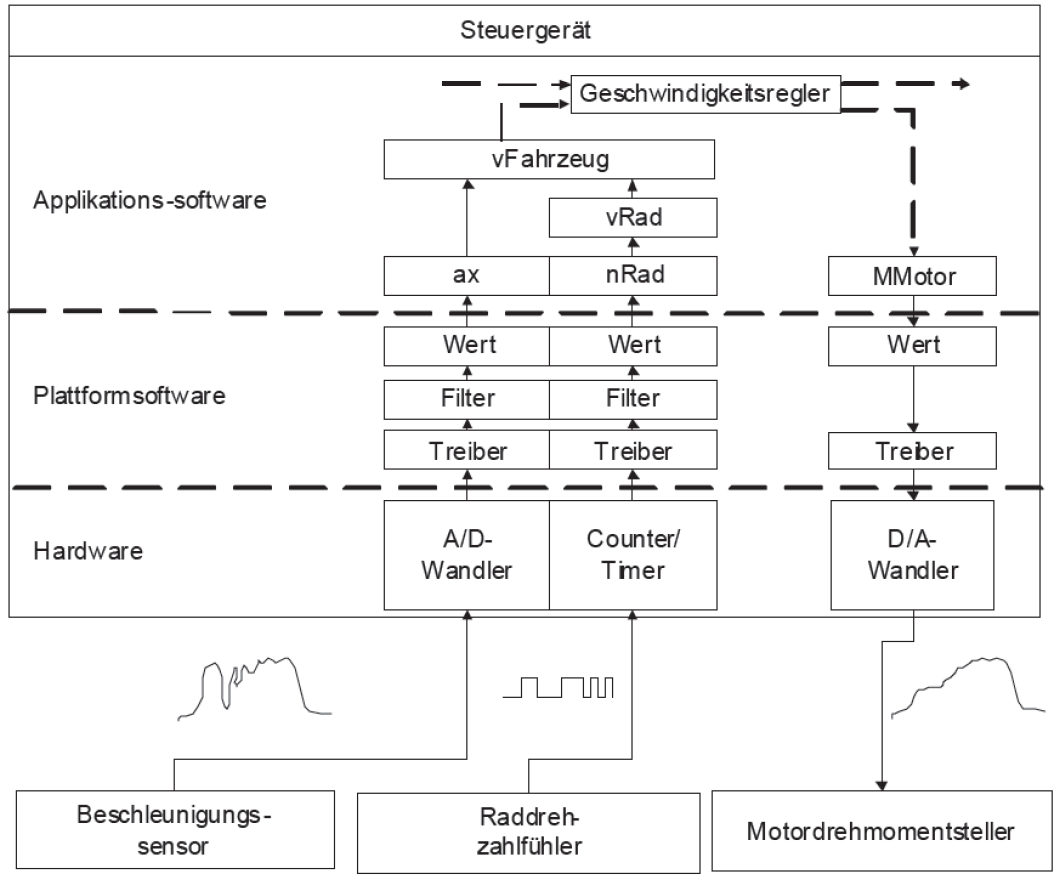
\includegraphics[width=0.8\columnwidth]{images/embedded_system_aufbau_schichten.png}
\end{center}


\subsection{Beispiele}

\vspace{-0.2cm}

\begin{minipage}[t]{0.48\columnwidth}
    \raggedright
    \subsubsection*{Fahrrad-Computer}

    \begin{outline}
        \1 GPS-Navigation
        \1 Geschwindigkeits- und Trittfrequenzmessung
        \1 Pulsmesser
        \1 Drahtlosübertragung (ANT+)
        \1 Interface zu elektronischer Gangschaltung
        \1 Barometer, Thermometer
        \1 Trainingsassistent
        \1 Display
    \end{outline}

    \subsubsection*{Weitere Beispiele}

    \begin{itemize}
        \item Smartphone
        \item Mobile Base Station
        \item CNC-Bearbeitungszentdrum
        % \item Schubumkehr bei Flugzeugen
        % \item Lungenzustandsdetektion mit Elektro-Impedanztomographie (EIT)
        \item Hörgerät
    \end{itemize}
\end{minipage}
\hfill
\begin{minipage}[t]{0.48\columnwidth}
    \raggedright
    \subsubsection*{Auto}

    \begin{outline}
        \1 Sicherheitsrelevante Aufgaben
            \2 ABS, ASR
            \2 Motorenregelung
            \2 Drive-by-wire
            \2 Autonom fahrende Autos
        \1 Unterhaltung / Komfort
            \2 Radio / CD / etc.
            \2 Navigation
            \2 Klima
        \1 Mehrere Netzwerke
            \2 CAN, LIN, Ethernet
        \1 Echtzeitteile und andere
        \1 Von einfachsten $\micro$Cs bis DSPs und GPUs 
    \end{outline}

    \textrightarrow\ Auto ist ein riesiges Embedded System
\end{minipage}


\subsection{Deeply Embedded System}

\begin{itemize}
    \item 'Einfaches' Embedded System, mit \textbf{minimaler Benutzerschnittstelle}, üblicherweise mit \textbf{keinerlei GUI}
        und \textbf{ohne Betriebssystem}
    \item Beschränkt auf \textbf{eine} Aufgabe (z.B. Regelung eines physikalischen Prozesses)
    \item Muss oft zeitliche Bedingungen erfüllen \textrightarrow\ Echtzeitsystem
\end{itemize}


\subsubsection{Beispiele -- Deeply Embedded System}

\begin{minipage}[t]{0.3\columnwidth}
    \begin{itemize}
        \item Hörgerät
        \item Motorenregelung
    \end{itemize}
\end{minipage}
\hfill
\begin{minipage}[t]{0.3\columnwidth}
    \begin{itemize}
        \item ABS-Controller
        \item 'Sensor' im IoT
    \end{itemize}
\end{minipage}
\hfill
\begin{minipage}[t]{0.3\columnwidth}
    \begin{itemize}
        \item etc...
    \end{itemize}
\end{minipage}


\subsection{Betriebssysteme bei Embedded Systems}

\begin{outline}
    \1 Es kommen Betriebssysteme wie (Embedded) Linux oder Android zum Einsatz \\
        \textrightarrow\ \textbf{Achtung: Linux und Android sind nicht echtzeitfähig!}
    \1 Wenn Echtzeit verlangt wird: real-time operating systems (RTOS)
        \2 Beispiele: Zephyr, Free RTOS (Amazon), TI-RTOS (Texas Instuments), etc. \\
            \textrightarrow\ RTOS siehe Abschnitt \ref{Real-Time Operating Systems (RTOS)}
\end{outline}


\subsection{Bare Metal Embedded System}

\begin{itemize}
    \item Es kommt \textbf{keinerlei Betriebssystem} zum Einsatz
    \item Bare Metal Embedded Systems sind recht \textbf{häufig}, insbesondere bei \textbf{Deeply Embedded Systems}
    \item Bare Metal Embedded Systems stellen besondere Ansprüche an Programmierung
\end{itemize}


\subsection{Zuverlässigkeit}

\begin{minipage}[c]{0.45\columnwidth}
    \pgfplotsset{samples=100}   % sample points to make graph smooth

\begin{center}
    \begin{tikzpicture}
        [
            scale = 0.6,
            >=latex
        ]
        \begin{axis}
            [
                title=\textbf{Zuverlässigkeit},
                width=8cm,
                height=5cm,
                xmin=-0.2, xmax=8, ymin=-0.1, ymax=1.3, axis lines=middle,
                x label style={at={(axis description cs:0.5,0)},anchor=north},
                y label style={at={(axis description cs:-0.1,0.5)},rotate=90,anchor=south},
                xlabel=Zeit,
                ylabel=Wahrscheinlichkeit,
                xtick=\empty,
                ytick={0, 0.2, 0.4, 0.6, 0.8, 1, 1.2}
                %grid
            ]
        
            % plot
            \addplot[color=blue, thick, domain=-0:10]{exp(-0.5*x)};
        \end{axis}
        
    \end{tikzpicture}
\end{center}
\end{minipage}
\hfill
\begin{minipage}[c]{0.5\columnwidth}
    \raggedright

    \begin{itemize}
        \item Je länger das System läuft, desto weniger zuverlässig ist es
        \item Die Wahrscheinlichkeit für einen Ausfall steigt stetig
    \end{itemize}
    
    \vspace{0.2cm}

    \textbf{Achtung:} Hier ist nur die Alterung der Hardware berücksichtigt
\end{minipage}


\subsection{Verfügbarkeit}

Die Verfügbarkeit A (availability) ist der Anteil der Betriebsdauer innerhalb dessen das System seine Funktion erfüllt.
$$ \text{Verfügbarkeit} = \frac{\text{Gesamtzeit} - \text{Ausfallzeit}}{\text{Gesamtzeit}} $$


% \subsection{Abstraktionsschichten}

% \begin{itemize}
%     \item Bei $\micro$C-Programmierung (Firmware) müssen oft Bitmuster in Register geschrieben werden
%     \item Solche Register-Zugriffe dürfen \textbf{nicht} 'willkürlich' überall im Code erfolgen \\
%         \textrightarrow\ schlecht lesbar, schlecht portiertbar, fehleranfällig
%     \item \textbf{Damit Code lesbarer und besser auf andere Platform portierbar wird, beinhaltet jeder professionelle Code einen
%         Hardware Abstraction Layer (HAL)}
%     \item HAL führt \textbf{nicht} zum Verlust bei Laufzeit, wenn korrekt implementiert
% \end{itemize}


% \subsubsection{Hardware-abstraction-layer (HAL)}

% \begin{itemize}
%     \item Trennt HW-Implementierung von SW-Logik
%     \item Gleiche SW kann auf verschiedene HW verwendet werden \textrightarrow\ Portabilität
%     \item HW-Komponenten können einfach ausgetauscht werden \textrightarrow\ Flexibilität
% \end{itemize}


        % % Modellierung von Embedded (real-time) Systems (Model Driven Development, MDD)
        % \section{Real-Time System (Echtzeitsystem)}

\subsection{Definitionen}

\subsubsection{Real-Time System (Echtzeitsystem)}

\begin{itemize}
    \item Ein Echtzeitsystem ist ein System, das Informationen \textbf{innerhalb einer definierten Zeit (deadline) bearbeiten} muss. \\
        \textrightarrow\ Explizite Anforderungen an \textbf{turnaround-time} (Antwortzeit) müssen erfüllt sein
    \item Wenn diese Zeit nicht eingehalten werden kann, ist mit einer \textbf{Fehlfunktion} zu rechnen.
\end{itemize}

\vspace{0.2cm}

\begin{minipage}[t]{0.55\columnwidth}
    \begin{center}
        \myul{\textbf{Typisches Echtzeitsystem}}

        \vspace{0.1cm}

        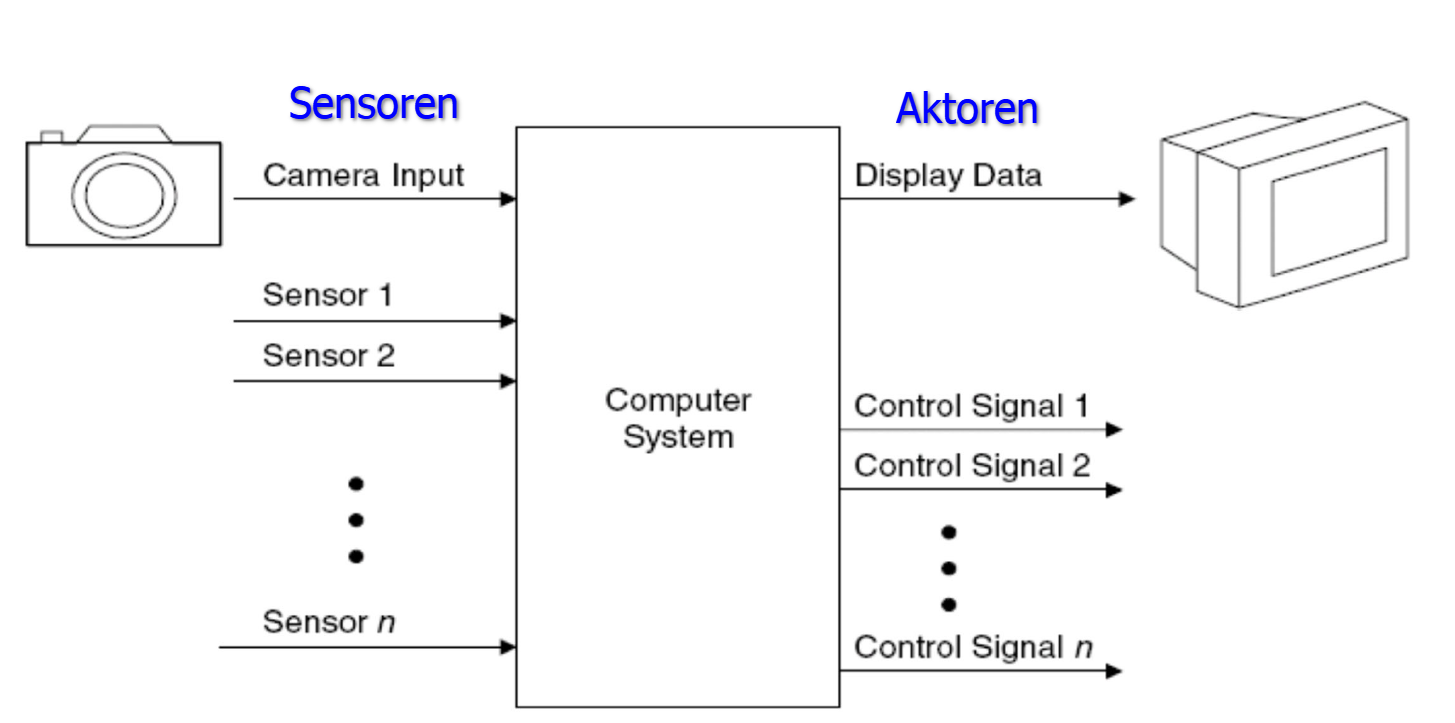
\includegraphics[width=\columnwidth]{images/typisches_echtzeitsystem.png}
    \end{center}
\end{minipage}
\hfill
\begin{minipage}[t]{0.4\columnwidth}
    \begin{center}
        \myul{\textbf{Repräsentation RT-System}}

        \vspace{0.1cm}

        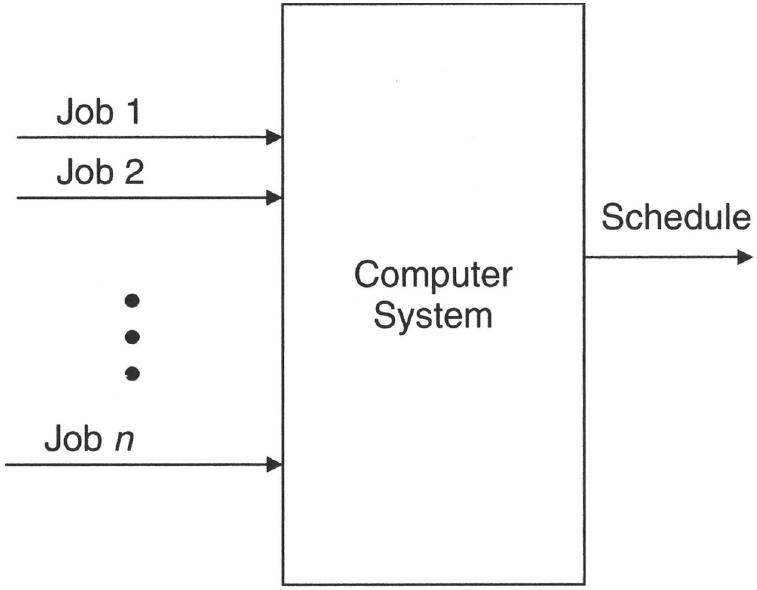
\includegraphics[width=0.7\columnwidth]{images/typische_repraesentation_echtzeitsystem.png}

        Sequenz von Aufgaben (Jobs) müssen zeitlich geplant (scheduled) werden
    \end{center}
\end{minipage}



\subsubsection{Zeitdefinitionen (Task)}

\begin{center}
    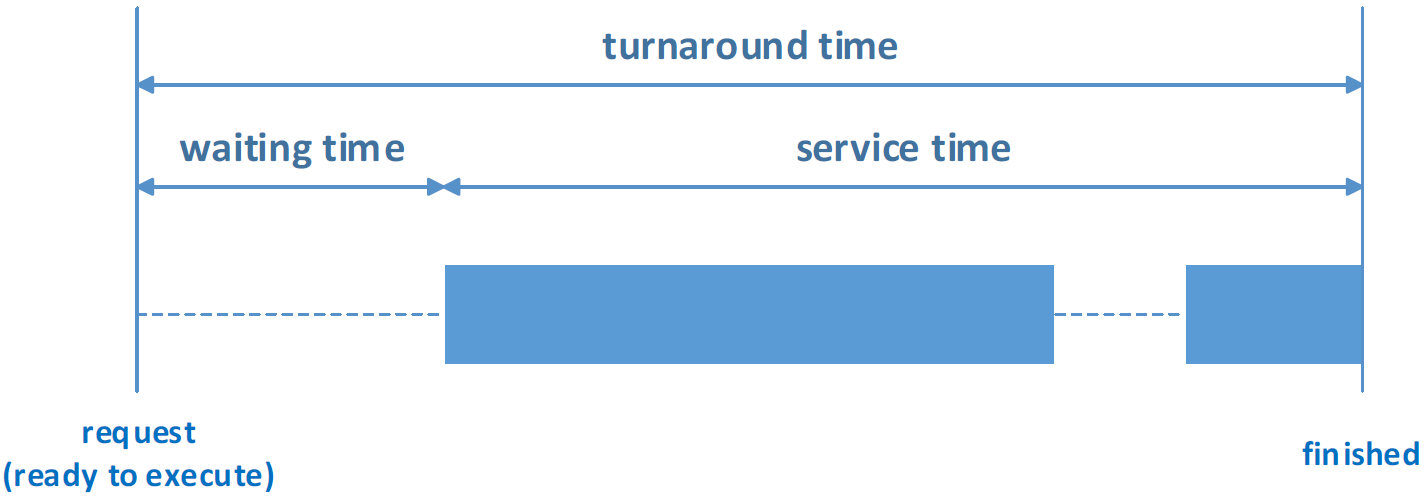
\includegraphics[width=0.7\columnwidth]{images/zeitdefinitionen_task.png}
\end{center}

\begin{outline}
    \1 \textbf{turnaround time:} (response time, Antwortzeit) 
        \2 Startet, wenn der Task bereit zur Ausführung ist und endet, wenn der Task fertig abgearbeitet ist
        \2 Zeit zwischen dem Vorhandensein von Eingangswerten an das System (Stimulus) bis zum Erscheinen der gewünschten Ausgangswerte.
    \1 \textbf{waiting time:} (Wartezeit)
        \2 Zeit zwischen Anliegen der Eingangswert und Beginn der Abarbeitung des Tasks
    \1 \textbf{service time:} (Bearbeitungszeit)
        \2 Zeit für Abarbeitung des Tasks \textrightarrow\ Unterbrechungen bzw. (preemptions) möglich 
\end{outline}


\subsection{Fehlverhalten eines Systems (failed system)}

\begin{itemize}
    \item Ein fehlerhaftes System (failed system = missglücktes System) ist ein System, das nicht alle formal
        definierten Systemspezifikationen erfüllt.
    \item \textbf{Die Korrektheit eines RT Systems bedingt sowohl die Korrektheit der Outputs als auch die Einhaltung
        der zeitlichen Anforderungen.}
\end{itemize}


\subsection{Echtzeitdefinition -- Verschiedene Echtzeitsysteme}

\begin{outline}
    \1 \textbf{soft real-time system} (weiches Echtzeitsystem)
        \2 Durch Verletzung der Antwortzeiten wird das System \textbf{nicht} ernsthaft beeinflusst
        \2 Es kommt zu Komforteinbussen
    \1 \textbf{hard real-time system} (hartes Echtzeitsystem)
        \2 Durch Verletzung der Antwortzeiten wird das \textbf{System ernsthaft beeinflusst}
        \2 Es kann zu einem kompletten Ausfall oder katastrophalem Fehlverhalten kommen
    \1 \textbf{firm real-time system} (festes Echtzeitsystem)
        \2 Kombination aus soft real-time system und hard real-time system
        \2 Durch Verletzung einiger weniger Antwortzeiten wird das System nicht ernsthaft beeinflusst
        \2 Bei vielen Verletzungen der Antwortzeiten kann es zu einem kompletten Ausfall oder katastrophalem Fehlverhalten kommen
\end{outline}


\subsubsection{Beispiele verscheidener Echtzeitsysteme}

\begin{center}
    \begin{tabular}{@{}lll@{}}
        \toprule
        \textbf{System}     & \textbf{Klassifizierung}  & \textbf{Erlärung}                             \\
        \midrule
        Geldautomat         & soft                      & Auch wenn mehrere Deadlines nicht eingehalten \\
                            &                           & werden können, entsteht dadurch keine         \\
                            &                           & Katastrophe. Im schlimmsten Fall erhält ein   \\
                            &                           & Kunde sein Geld nicht.                        \\
        \midrule
        GPS-gesteuerter     & firm                      & Wenn die Positionsbestimmung versagt, könnte  \\
        Rasenmäher          &                           & das Blumenbeet der Nachbarn platt gemäht      \\
                            &                           & werden.                                       \\
        \midrule
        Regelung eines      & hard                      & Das Versagen der Regelung kann dazu führen,   \\
        Quadrocopters       &                           & dass der Quadrocopter ausser Kontrolle        \\
                            &                           & gerät und abstürzt.                           \\
        \bottomrule
    \end{tabular}
\end{center}


% \subsection{Determinsismus (determinacy)}


% \subsection{Auslastung (utilization)}


% \subsection{Real-time Scheduling}

        % \section{Modellierung eines Embedded Systems}

\subsection{V-Modell für Software-Entwicklungszyklus}

\begin{center}
    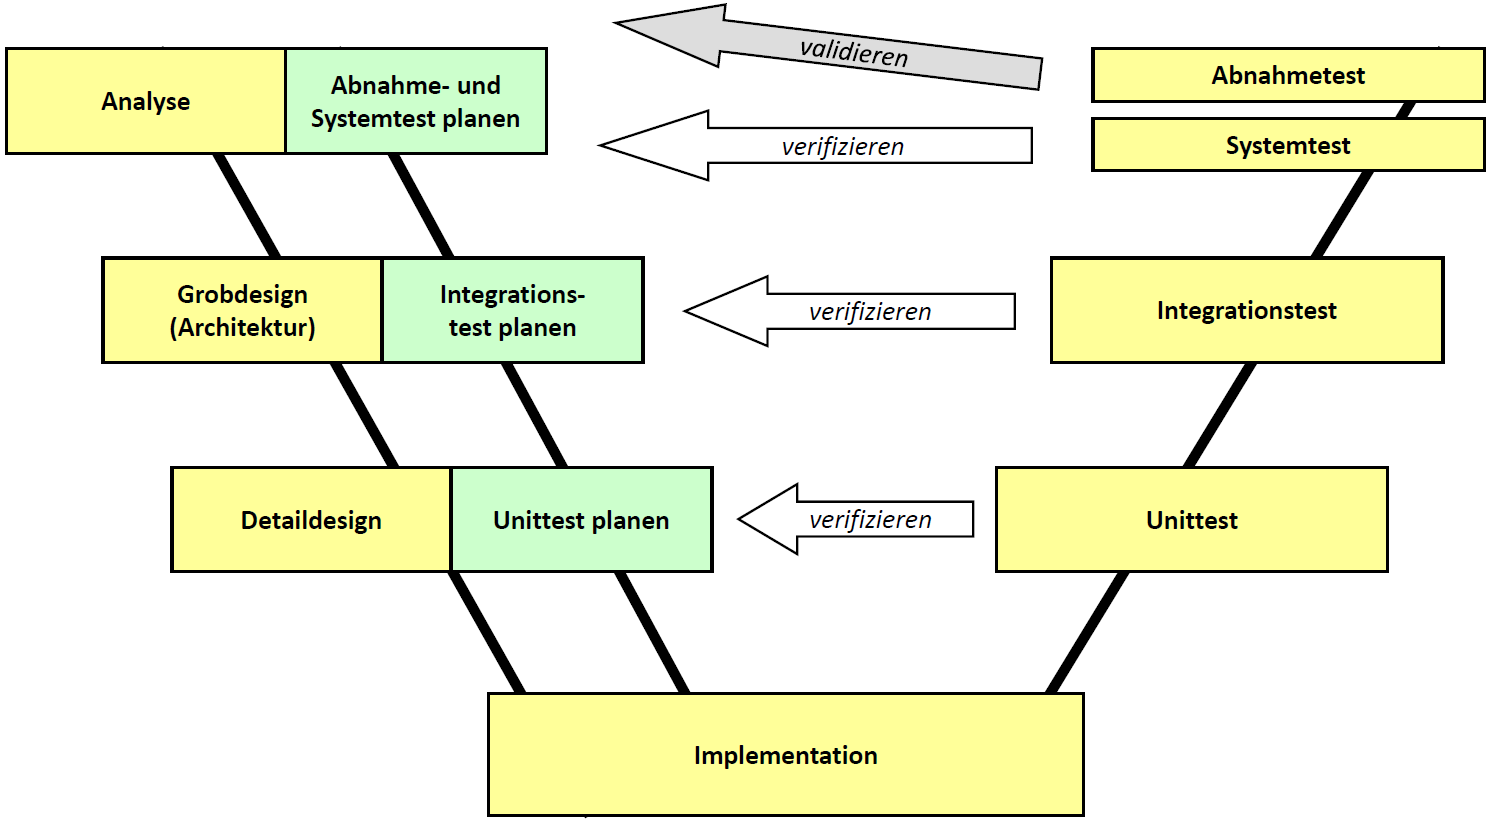
\includegraphics[width=0.7\columnwidth]{images/V_modell.png}
\end{center}

\textrightarrow\ Nur Anforderungen (requirements) definieren, welche man auch testen kann!


\subsection{Model Driven Development (MDD)}

\begin{outline}
    \1 Bei \textbf{modellbasierter Entwicklung} kommen in \textbf{allen Entwicklungsphasen} durchgängig Modelle zum zur Anwendung
    \1 MDD geht davon aus, dass aus formalen Modellen lauffähige Software erzeugt wird \\
        \textrightarrow\ Codegeneratoren
    \1 Modelle werden traditionell als Werkzeug der Dokumentation angesehen
        \2 Unter Umständen wird zweimal dasslbe beschrieben (Code und Diagramm) \\
            \textbf{\textrightarrow\ unbedingt zu vermeiden!}
\end{outline}


\subsection{Vorgehen bei der Modellierung}

\begin{minipage}[c]{0.6\columnwidth}
    \begingroup
    \renewcommand{\outlinei}{enumerate}
    \renewcommand{\outlineii}{itemize}

    \begin{outline}
        \1  \cgn{Systemgrenze definieren}
            \2 Kontextdiagramm: Use-Case-Diagramm
            \2 Kontextdiagramm: Sequenzdiagramm
        \1 \cgn{Systemprozess finden}
            \2 Kontextdiagramm: Use-Case-Diagramm
            \2 Kontextdiagramm: Sequenzdiagramm
        \1 \cgn{Verteilungen festlegen}
            \2 Verteilungsdiagramm (deployment diagram)
        \1 \cbl{Systemprozesse detaillieren}
            \2 Umgangssprachlicher Text
            \2 Sequenzdiagramm
            \2 Aktivitätsdigramm
            \2 Statecharts
            \2 Code (C, C++, ...)
    \end{outline}
    \endgroup
\end{minipage}
\hfill
\begin{minipage}[c]{0.38\columnwidth}
    \raggedright
    \cgn{Stukturmodellierung (Statische Aspekte)}
    
    \vspace{0.2cm}

    \cbl{Modellierung der dynamischen Aspekte}
\end{minipage}


\subsection{Systemgrenze definieren \& Systemprozesse finden}

\subsubsection{Systemgrenze definieren}

\textbf{Die Festlegung der Systemgrenze ist das Wichtigste und Allererste bei sämtlichen Systemen!}

Man sollte sich die folgenden Fragen stellen und diese beantworten:

\vspace{0.1cm}

\begin{outline}
    \1 Was macht das System, d.h. was liegt innerhalb der Systemgrenze?
        \2 Was macht das System  \textbf{nicht}?
    \1 Mit welchen Teilen ausserhalb des Systems kommuniziert das System?
    \1 Welches sind die Schnittstellen zu den Nachbarsystemen (Umsystemen, periheral system)?
\end{outline}


\subsubsection{Systemprozesse finden (use-cases)}

Da man sich noch immer in der \textbf{Analyse} befindet, sollen nur die \textbf{Anforderungen} definiert werden. Die Umsetzung ist Teil
des Designs! \\
Um die Use-Cases zu identifizieren, sollte folgendes beachtet werden:

\vspace{0.1cm}

\begin{outline}
    \1 Aussenbetrachtung des Systems (\textbf{oberflächlich!})
        \2 Nicht komplizierter als nötig
    \1 System als Blackbox betrachten 
        \2 \textbf{Was} soll System können; (nicht: wie soll das System etwas machen)
    \1 RTE-Systeme bestehen häufig aus nur einem einzigen Systemprozess 
        \2 speziell wenn System 'nur' ein Regler ist
\end{outline}


\subsubsection{Kontextdiagramm: Use-Case Diagramm}

\begin{minipage}[t]{0.4\columnwidth}
    \myul{\textbf{Tempomat: zu detailliert}}

    \vspace{0.1cm}

    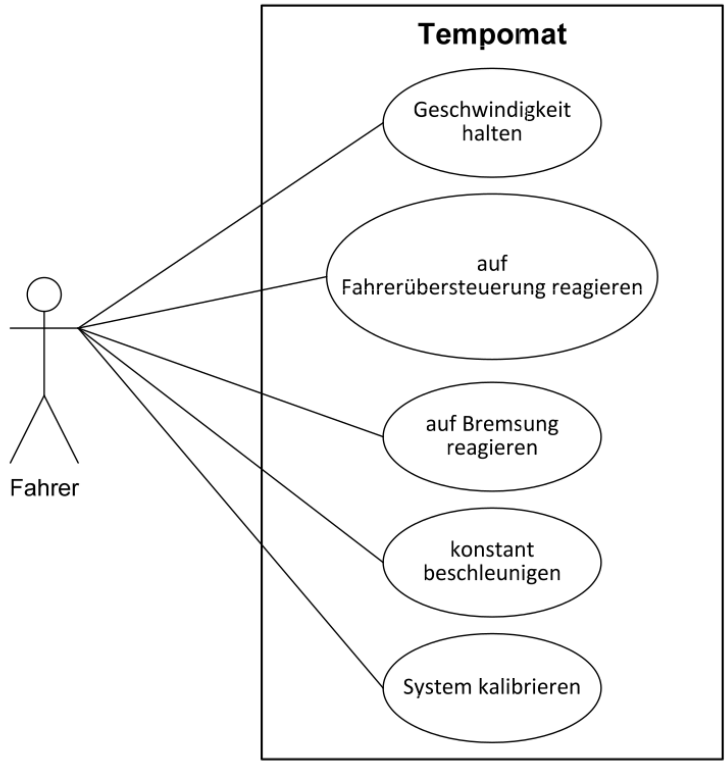
\includegraphics[width=\columnwidth]{images/use-case-diagramm_schlecht.png}
\end{minipage}
\hfill
\begin{minipage}[t]{0.48\columnwidth}
    \myul{\textbf{Tempomat: verbesserte Version}}

    \vspace{0.1cm}

    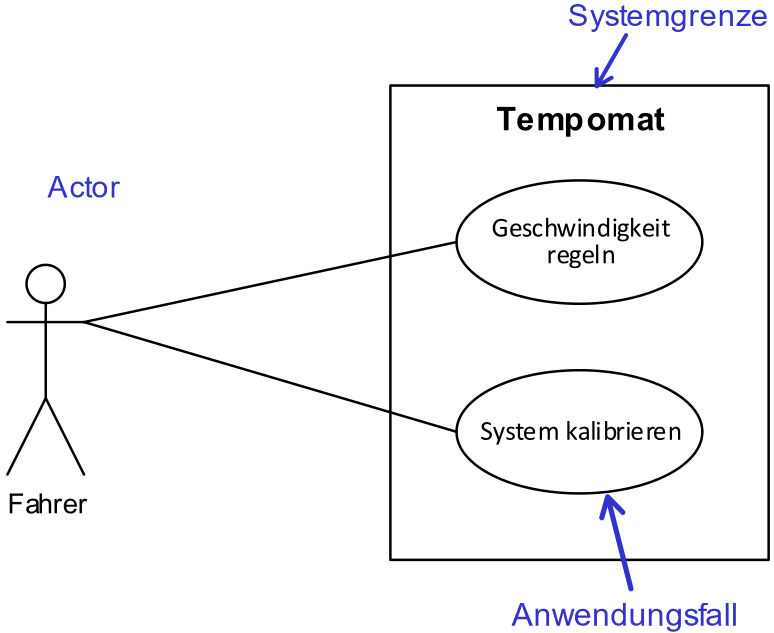
\includegraphics[width=\columnwidth]{images/use-case-diagramm_besser.png}
\end{minipage}


\subsubsection{Kontextdiagramm: Sequenzdiagramm}

\begin{itemize}
    \item Speziell bei Syetemen, deren Grenzen durch \textbf{Nachrichtenflüsse} charakterisiert werden können
    \item Details zu Sequenzdiagrammen siehe Abschnitt % TODO
\end{itemize}


\subsection{Verteilungen festlegen}

\begin{itemize}
    \item Bei Embedded Systems werden häufg \textbf{mehrere Rechnersysteme} verwendet, um die verschiedenen Aufgaben zu erledigen
    \item Rechner sind örtlich verteilt und mittels Kommunikationskanal verbunden \\
        \textbf{\textrightarrow\ Verteilte Systeme (distributed systems)}
\end{itemize}

\vspace{0.2cm}

\begin{minipage}[t]{0.5\columnwidth}
    \raggedright

    \subsubsection{Verteilungsdiagramm}
    
    \begin{description}
        \item[Knoten:] Darstellung der örtlichen Verteilung der Systeme \\
            Knoten können auch hierarchisch aufgebaut sein
        \item[Linien:] Physikalische Verbindungen der Knoten (Netzwerke, Kabel, Wireless, etc.)
    \end{description}
\end{minipage}
\hfill
\begin{minipage}[t]{0.46\columnwidth}
    \example{Tempomat}
    
    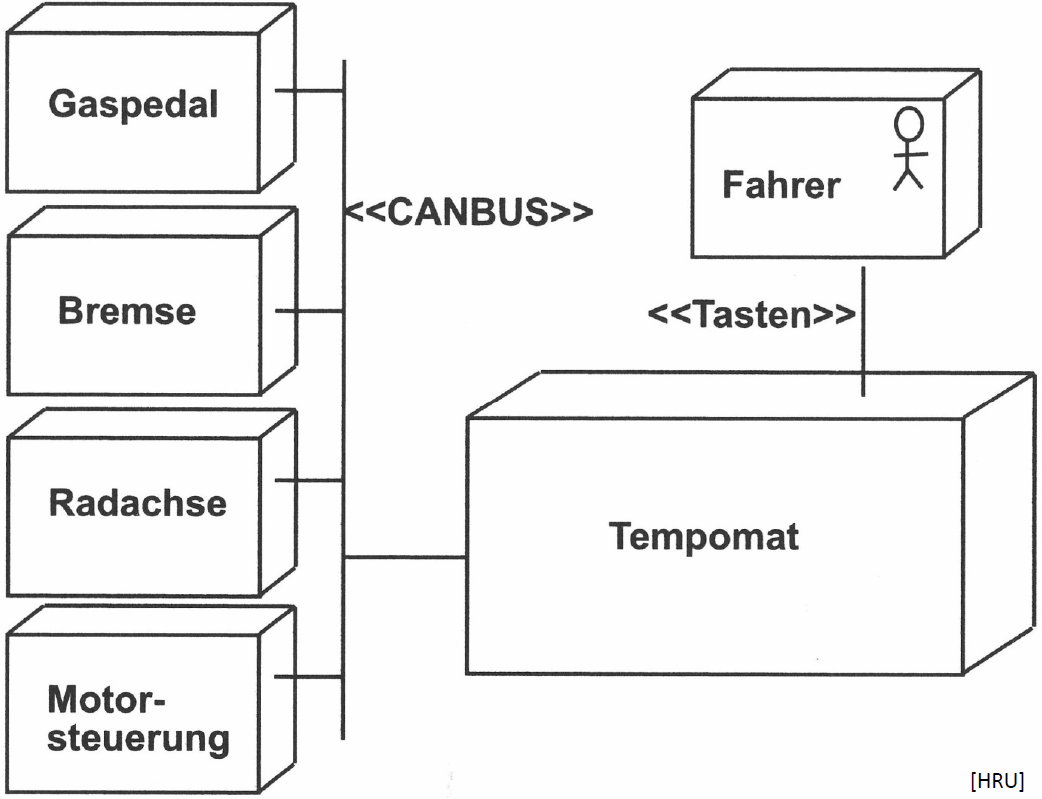
\includegraphics[width=\columnwidth]{images/verteilungsdiagramm_tempomat.png}
\end{minipage}


\subsection{Systemprozesse detaillieren}

\begin{outline}
    \1 Die gefundenen Systemprozesse (use-cases) müssen genauer spezifiziert werden
        \2 \textbf{Nicht detaillierter spezifizieren als sinnvoll / gefordert!}
        \2 Jede weitere Spezifizierung soll eien 'added value' liefern
    \1 Verschiedene Detaillierungsstufen für verschiedene Zielgruppen
        \2 Auftraggeber: Überblick (z.B. in Form von Umgangssprachlichem Text)
        \2 Systementwickler: 'Normale Sicht' enthält mehr Details
\end{outline}


\subsubsection{Sequenzdiagramm}


        % % Hardware/Software Codesign
        % \section{Hardware-Software-Codesign}

\subsection{Ziele}

\begin{itemize}
    \item Entwurf (Design) \textbf{so lange wie sinnvoll} (nicht so lange wie möglich) \textbf{lösungsneutral}
    \item \textbf{Systemdesign fördern}, statt separate Designs für Mechanik, Elektronik, Firmware, Software, etc., die sich
        unter Umständen auch widersprechen können
    \item Systemspezifikation erfolgt idealerweise mit Hilfe einer \textbf{eindeutigen Spezifikationssprache}, nicht in
        Prosa
    \item Die Spezifikation sollte simuliert (ausgeführt) werden können
    \item Implementationen können einfach geändert werden: HW \textlrarrow\ SW
    \item Zielplattformen: diskrete Elektronik, ASIC, \textmu C, DSP, \textbf{FPGA}, Software
\end{itemize}


\subsection{Anforderungen für praktische Anwendungen}

\begin{outline}
    \1 Methoden / Tools sollten beim Systemdesign nicht zu fachlastig sein
        \2 Methoden sollten für Elektronik-, Firmware- und wenn möglich auch Mechanikentwickler anwendbar sein
    \1 Wenn möglich gute Toolunterstützung
    \1 (Automatische Synthese aus dem Modell)
\end{outline}


\subsection{Spezifikationssprachen}

\begin{minipage}[t]{0.48\columnwidth}
    \raggedright
    \begin{itemize}
    \item \textbf{Formale Sprachen sind eindeutig} \\
        (Prosa immer mehrdeutig)
    \item Spezifikation kann compiliert und ausgeführt werden \textrightarrow\ Simulationen
    \item Die ausführbare Spezifikation dient als \textbf{Golden Reference} für die künftigen Entwicklungsschritte
\end{itemize}
\end{minipage}
\hfill
\begin{minipage}[t]{0.48\columnwidth}
    \myul{\textbf{Beispiele für Spezifikationssprachen}}

    \vspace{0.1cm}

    \begin{itemize}
        \item SystemC (eine C++-Template Library)
        \item SysML
        \item SpecC
        \item SystemVerilog
        \item Esterel
        \item Matlab/Simulink
        \item Statecharts
    \end{itemize}
\end{minipage}


\subsection{Virtuelle Prototypen}

\begin{itemize}
    \item Die Simulation des Systems kann unterschiedlich stark detailliert werden
    \item \textbf{Die simulierten Systeme sind Virtuelle Prototypen}
    \item Während der Entwicklung können einzelne (virtuelle) Teile des Prototyps laufend durch physische Teile
        ersetzt werden
\end{itemize}


\subsection{X-in-the-loop}

\begin{outline}
    \1 \textbf{Model-in-the-Loop (MIL):} Vollständig als Modell vorliegender virtuellen Prototyp
    \1 Je mehr der Prototyp durch konkretere Implementationen ersetzt wird, spricht man von
        \2 Software-in-the loop (SIL)
        \2 Processor-in-the loop (PIL)
        \2 Hardware-in-the loop (HIL)
\end{outline}

\vspace{0.2cm}

\textrightarrow\ Test outputs werden jeweils mit \textbf{Golden Reference} verglichen
\begin{center}
    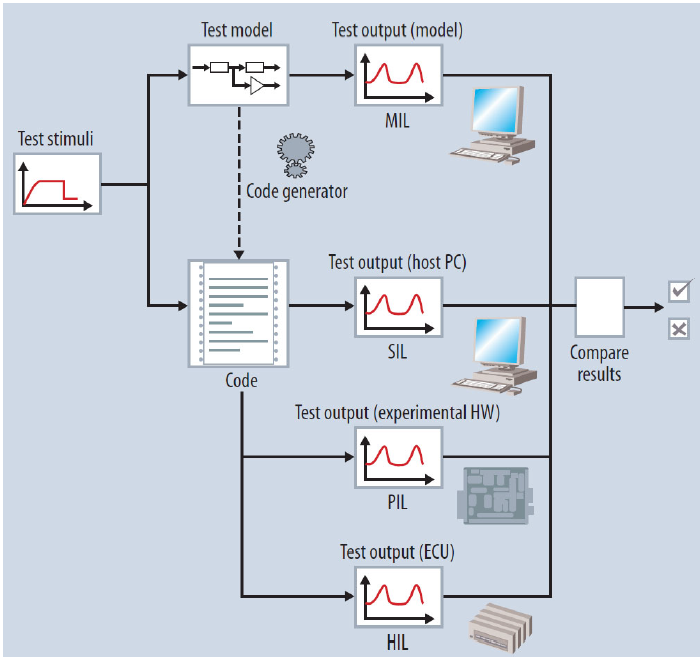
\includegraphics[width=0.9\columnwidth]{images/x_in_loop_testing.png}
\end{center}


\subsection{Entwicklungsplattformen}

Als Entwicklungsplattformen eignen sich häufig \textbf{FPGA basierte Systeme.}

\begin{outline}
    \1 Hardware mit VHDL
    \1 Software/Firmware in C/C++
        \2 auf integriertem \textmu C (z.B. Zynq von AMD/Xilinx) (Hard Core)
        \2 auf Soft Core innerhalb FPGA (z.B. Nios II von Intel/Altera)
\end{outline}


        % % Finite State Machines (Anwendung, Implementationen in C und C++)
        % \section{Zustandsbasierte Systeme}

\subsection{Asynchrone vs. synchrone FSM}

\begin{minipage}[t]{0.48\columnwidth}
    \raggedright
    \begin{outline}
        \1 \textbf{Asynchron}
            \2 geänderte Inputsignale führen \textbf{direkt} zur Zustandsänderung
            \2 schneller, aber enorm anfällig auf Glitches
    \end{outline}
\end{minipage}
\hfill
\begin{minipage}[t]{0.48\columnwidth}
    \raggedright
    \begin{outline}
        \1 \textbf{Synchron}
            \2 Inputsignale werden nur zu diskreten Zeitpunkten betrachtet \\
                \textrightarrow\ getaktete Systeme
    \end{outline}
\end{minipage}

\vspace{0.2cm}
%TODO: check if this is finished
\begin{outline}
    \1 Softwareimplementationen sind eigentlich immer \textbf{synchron}, da Rechner getaktet sind
    \1 Rein softwareseitig besteht die Problematik der Asynchronizität nicht
\end{outline}


\subsection{Finite State Machines (FSM)}


\subsubsection{Mealy-Automat}

\subsubsection{Moore-Automat}
% Bondi: alles als Moore modellieren

\subsubsection{Medvedjev}
%hier nicht weiter behandelt...?
% Zustand = Output


\subsection{State-Event-Diagramm (Zustandsdiagramm)}

% Beschreibung


\example{State-Event-Diagramm -- Moore Automat}

% \begin{center}
%     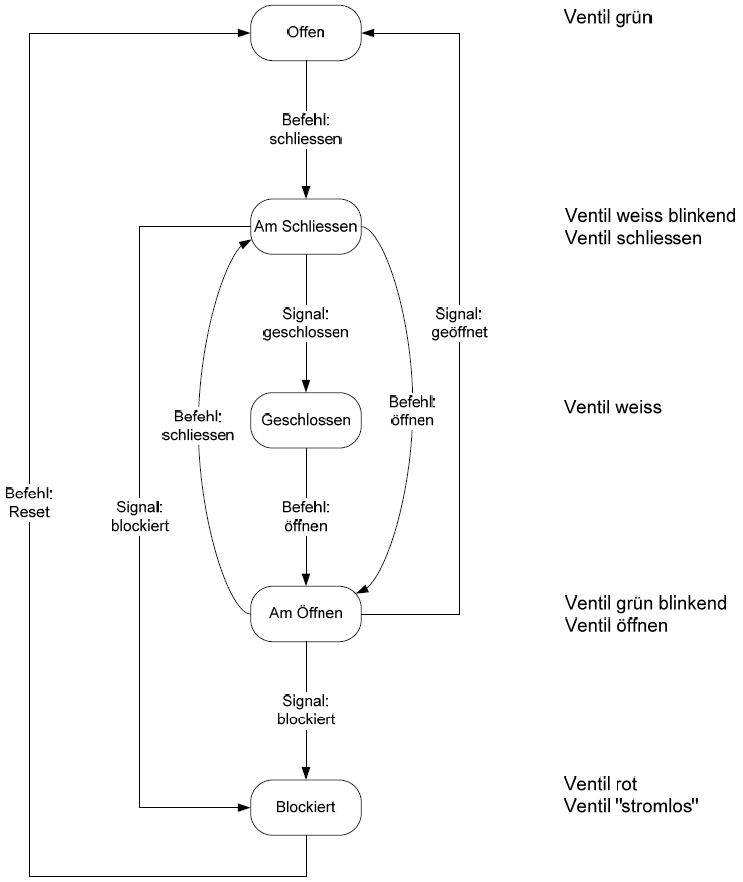
\includegraphics[width=0.8\columnwidth]{images/state_event_example.png}
% \end{center}


        % \section{Statecharts}

\subsection{Nachteile von State-Event-Diagrammen}

\begin{itemize}
    \item Zustandsdiagramme sind flach (es gibt keine Hierarchie) \textrightarrow\ schnell unübersichtlicht
    \item Es kann keine zeitliche Parallelität modelliert werden
\end{itemize}


\subsection{Definitionen}


\subsubsection{Elemehte der Statecharts}



\subsection{Hierarchie}


\subsection{Default-State}


\subsection{History}

\subsubsection{Shallow History}


\subsubsection{Deep History}



\subsection{Parallelität}


\subsection{Timers}



\subsection{Beispiel -- Armbanduhr als Statechart}  %CHECK: vielleicht gibt es im Praktikum ein besseres Beispiel...?


        % \section{Realisierung flache FSM}

\subsection{Mögliche Realisierungen von flachen FSMs}

\begin{outline}
    \1 Steuerkonstrukt (typischerweise mit \textbf{switch-case})
        \2 prozedural oder objektorientiert
    \1 Definition und Abarbeitung einer \textbf{Tabelle}
        \2 prozedural oder objektorientiert
    \1 \textbf{State Pattern} (Gang of Four, GoF)
        \2 nur objektorientiert
    \1 Generisch mit Templates
        \2 nur mit einer Sprache, die Templates unterstützt (z.B. C++)
\end{outline}

\vspace{0.2cm}

\textrightarrow\ Alle Varianten haben wie immer sowohl Vor- als auch Nachteile \\
\textrightarrow\ Bei allen Varianten sind auch Variationen vorhanden


\subsection{Realisieurng mit Steuerkonstrukt (prozedural in C)}

\subsubsection{State-Event-Diagram -- Up/Down-Counter}

\begin{center}
    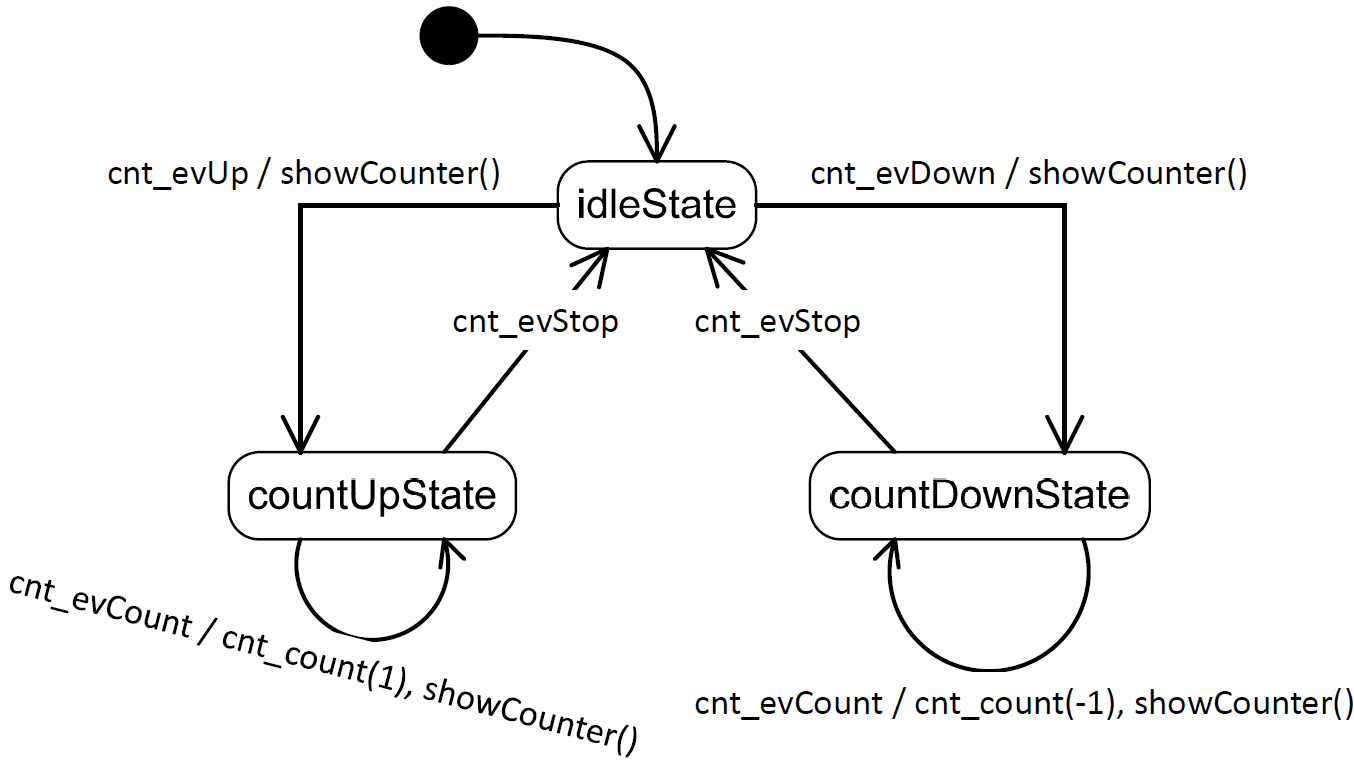
\includegraphics[width=0.7\columnwidth]{images/fsm_up-down-counter_diagramm_C.png}
\end{center}


\subsubsection{Implementation der Prozeduralen Realisierung in C}

\begin{outline}
    \1 \textbf{Ereignisse (events)}
        \2 Schnittstelle nach aussen \textrightarrow\ ändern Zustand der FSM
        \2 In enum definiert (\textbf{public}) \textrightarrow\ header-file
        \2 Einzelne Events und enum Bezeichnung enthalten \textbf{Unitkürzel} (hier: \mylstbox{cnt_})
    \1 \textbf{Zustände (states)}
        \2 In enum definiert (\textbf{nicht} public) \textrightarrow\ sourcecode-file
    \1 \textbf{Aktueller Zustand} wird in einer \textbf{statischen Varianlen} gehalten
    \1 Die FSM wird in \textbf{zwei Funktionen} implementiert
        \2 Initialiserungs-Funktion (hier: \mylstbox{void cnt_ctrlInit(int initValue)})
        \2 Prozess-Funktion (hier: \mylstbox{void cnt_ctrlProcess(cnt_Event e)}) \\
            \textrightarrow\ Zustände prüfen, Zustandsübergänge veranlassen
    \1 Anstossen einer FSM
        \2 Initialisierung in \lstinline|main|-Funktion
        \2 Überprüfung, welches Event aufgetreten ist meist in \mylstbox{do-while}-Schleife
\end{outline}


\subsubsection{Eigenschaften der Prozeduralen Realisierung in C}

\begin{outline}
    \1 Da aktueller Zustand eine statische Variable ist, kann es nur \textbf{eine einzige Instanz} der FSM geben
    \1 Bei mehreren Instanzen in C...
        \2 darf \mylstbox{currentState} nicht \mylstbox{static} sein und muss als Parameter mitgegenen werden,
            bzw. ein Pointer auf die jeweilige Variable
        \2 Zustands-enum muss in die Schnittstelle (header-file) oder es muss z.B. mit \mylstbox{void*} gearbeitet werden
    \1 In C ist \textbf{keine schöne Kapselung} der Attribute möglich (\mylstbox{currentState})
    \1 Funktion \mylstbox{cnt_ctrlProcess()} kann beliebig aufgerufen werden (periodischer Task, laufend, etc.)
    \1 Bei exponierten Funktionen / Definitionen muss in C ein Unitkürzel vorangestellt werden (hier: \mylstbox{cnt_})
\end{outline}


\example{Up/Down-Counter (prozedural in C)}

% TODO: \para environment not showing...?
% TODO: add keywords and stuff to listings setup

\begin{minipage}[t]{0.48\columnwidth}
    \para{Schnittstelle Counter in C} 
    \lstinputlisting{snippets/fsm_procedural_C/fsm_counter_C.h}
\end{minipage}
\hfill
\begin{minipage}[t]{0.48\columnwidth}
    \para{Implementation Counter in C} 
    \lstinputlisting{snippets/fsm_procedural_C/fsm_counter_C.c}
\end{minipage}


\para{Schnittstelle FSM in C} 
\lstinputlisting{snippets/fsm_procedural_C/fsm_counterCtrl_C.h} 

\para{Implementation FSM in C} 
\lstinputlisting{snippets/fsm_procedural_C/fsm_counterCtrl_C.c}

\para{Anstossen der FSM in C} 
\lstinputlisting{snippets/fsm_procedural_C/fsm_main_counterTest_C.c}



\subsection{Realisieurng mit Steuerkonstrukt (objektorientiert in C++)}
\label{Realisieurng mit Steuerkonstrukt (objektorientiert in CPP)}

\subsubsection{State-Event-Diagram -- Up/Down-Counter}
\label{State-Event-Diagram -- Up/Down-Counter in CPP}

\begin{center}
    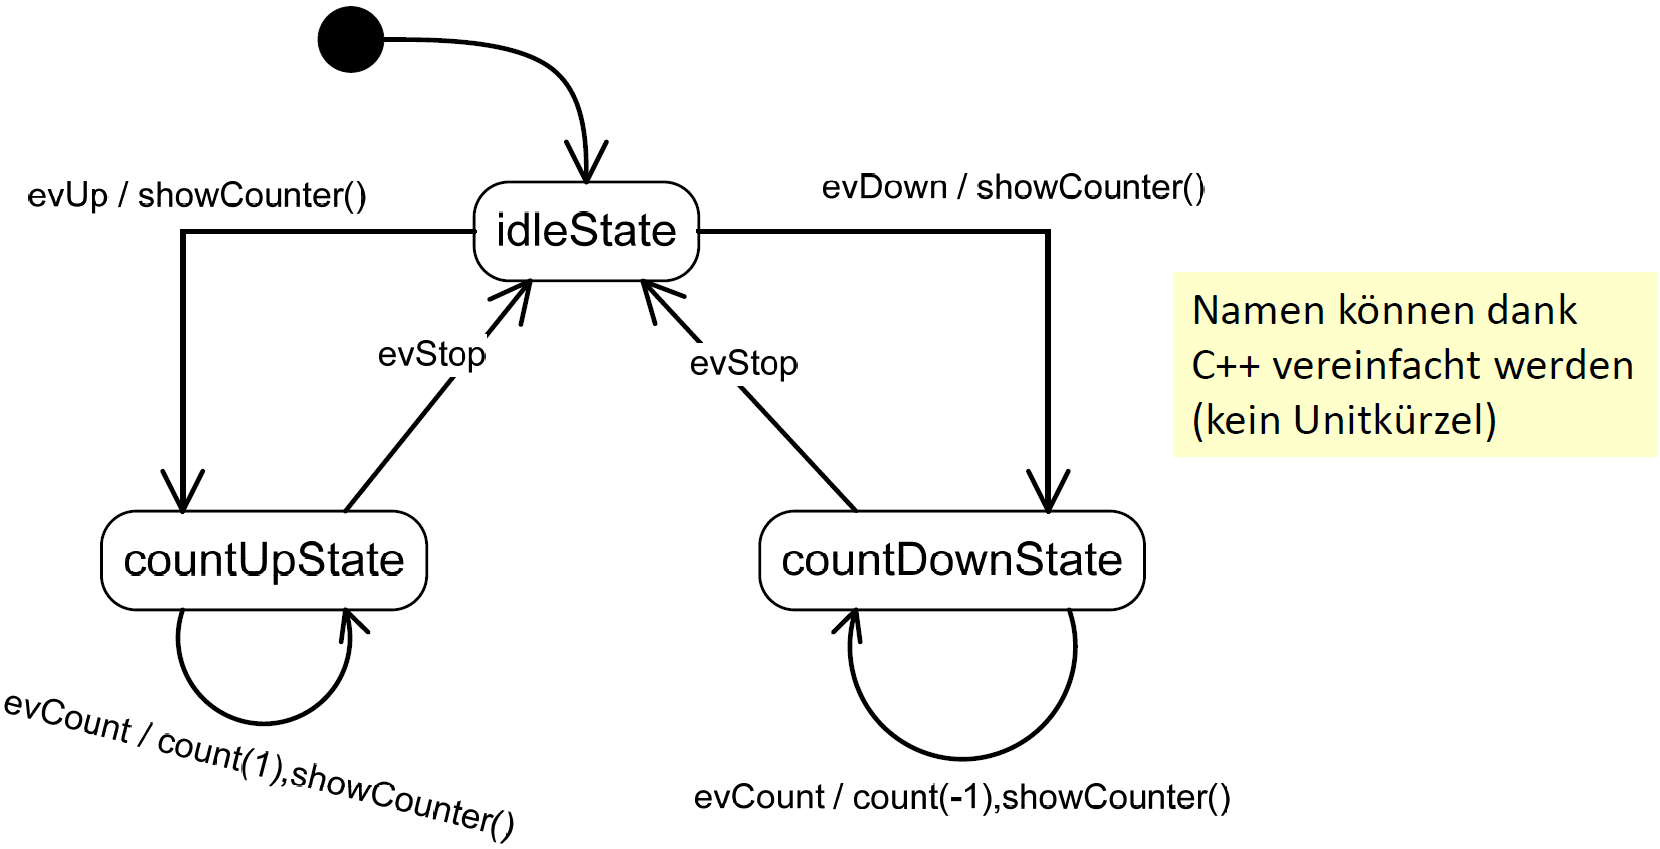
\includegraphics[width=0.7\columnwidth]{images/fsm_up-down-counter_diagramm_CPP.png}
\end{center}


\subsubsection{Zusammenhang der Klassen Counter und CounterCtrl}
\label{Zusammenhang der Klassen Counter und CounterCtrl}

\begin{center}
    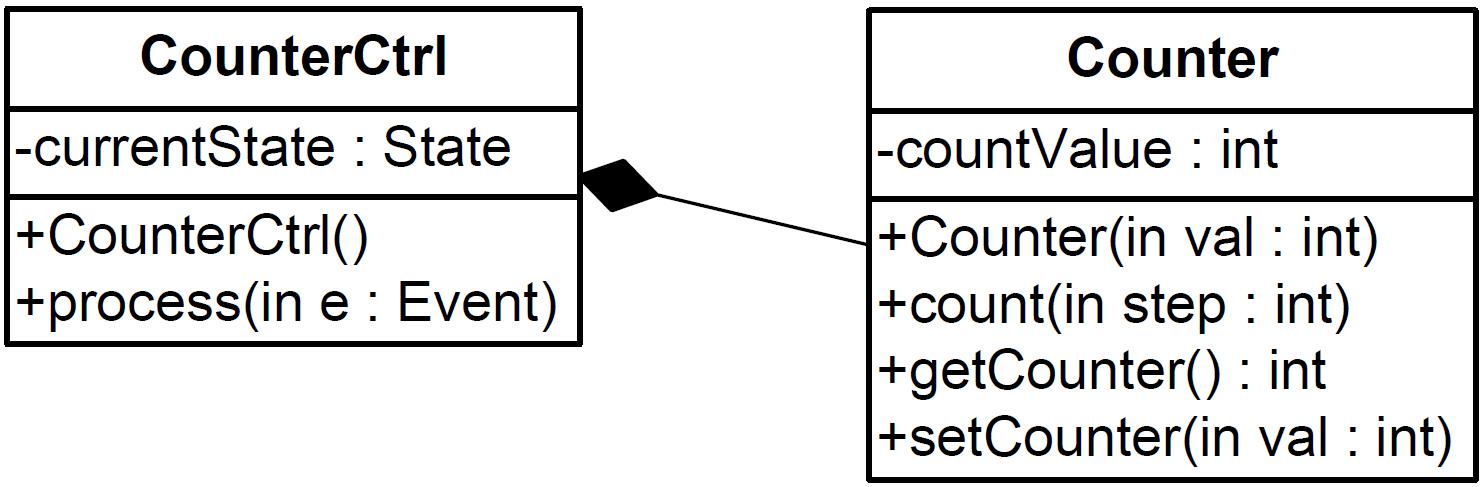
\includegraphics[width=0.7\columnwidth]{images/fsm_CPP_klassendiagramm.png}
\end{center}

\begin{outline}
    \1 Klasse \mylstbox{Counter} führt eigentliche Rechenaufgaben durch
        \2 ist bei \textbf{allen} (objektorientierten) Realiseurngsarten \textbf{identisch}
    \1 Klasse \mylstbox{CounterCtrl} ist FSM, welche Zugriff auf den Counter steuert 
\end{outline}

\textbf{ \textrightarrow\ Generell sollten Steuerung und Element, das gesteuert wird, getrennt werden!}


\subsubsection{Implementation der Prozeduralen Realisierung in C++}

\begin{outline}
    \1 \textbf{Ereignisse (events)}
        \2 Schnittstelle nach aussen \textrightarrow\ ändern Zustand der FSM
        \2 Im \textbf{public} Teil der Klasse als enum definiert
        \2 Keine Unitkürzel nötig
    \1 \textbf{Zustände (states)}
        \2 Im \textbf{private} Teil der Klasse als enum definiert \textrightarrow\ header-file
    \1 \textbf{Aktueller Zustand} \mylstbox{currentState} wird in \textbf{privatem Attribut} von \mylstbox{CounterCtrl} gehalten
    \1 Die FSM wird in \textbf{zwei Funktionen} implementiert
        \2 Kontruktor (hier: \mylstbox{CounterCtrl::CounterCtrl(int initValue=0)})
        \2 Prozess-Funktion (hier: \mylstbox{void CounterCtrl::process(CounterCtrl::Event e)}) \\
            \textrightarrow\ Zustände prüfen, Zustandsübergänge veranlassen
    \1 Anstossen einer FSM
        \2 Initialisierung in \lstinline|main|-Funktion
        \2 Überprüfung, welches Event aufgetreten ist meist in \mylstbox{do-while}-Schleife
\end{outline}


\example{Up/Down-Counter (prozedural in C++)}

% TODO: \para environment not showing...?
% TODO: add keywords and stuff to listings setup

\begin{minipage}[t]{0.44\columnwidth}
    \para{Schnitstelle Counter in C++} 
    \lstinputlisting{snippets/fsm_procedural_CPP/fsm_Counter_CPP.h}
\end{minipage}
\hfill
\begin{minipage}[t]{0.52\columnwidth}
    \para{Implementation Counter in C++} 
    \lstinputlisting{snippets/fsm_procedural_CPP/fsm_Counter_CPP.cpp}
\end{minipage}


\para{Schnittstelle FSM in C++} 
\lstinputlisting{snippets/fsm_procedural_CPP/fsm_CounterCtrl_CPP.h} 

\para{Implementation FSM in C++} 
\lstinputlisting{snippets/fsm_procedural_CPP/fsm_CounterCtrl_CPP.cpp}

\para{Anstossen der FSM} 
\lstinputlisting{snippets/fsm_procedural_CPP/fsm_main_counterTest_CPP.cpp}



\subsection{Realisierung mit Tabelle}

\subsubsection{State-Event-Diagram -- Up/Down-Counter}

Siehe Abschnitt \ref{State-Event-Diagram -- Up/Down-Counter in CPP}


\subsubsection{FSM in Tabellenform}

Das State-Event-Diagramm wird in eine Tabelle 'übersetzt'. \textbf{Jede Zeile der Tabelle entspricht einer Transition (Pfeil) im 
State-Event-Diagramm}

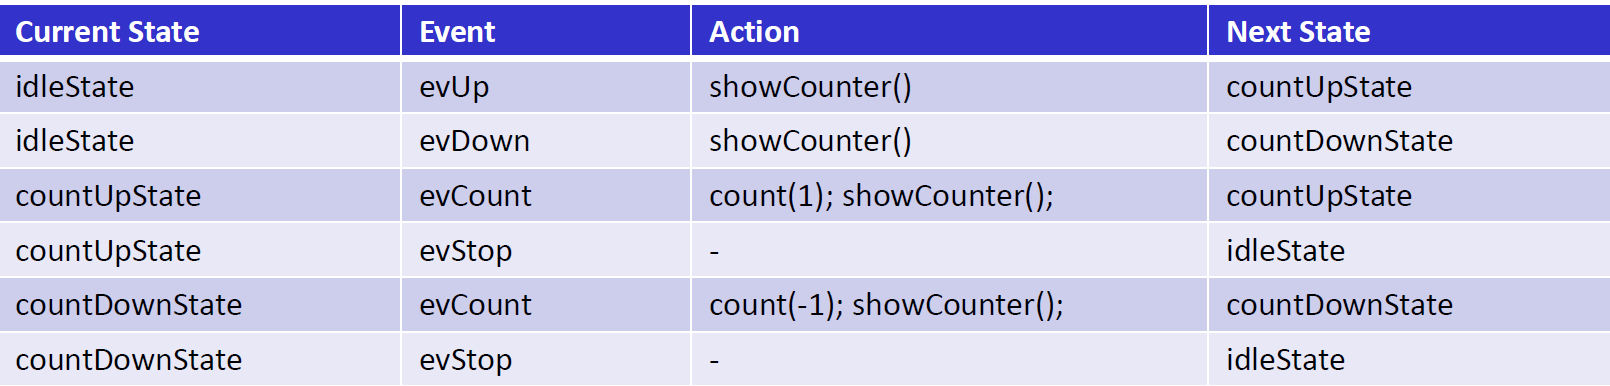
\includegraphics[width=\columnwidth]{images/fsm_tabelle.png}


\subsubsection{Implementation der Realisierung mittels Tabelle in C++}

\begin{outline}
    \1 Die ganze FSM ist in einer Tabelle gespeichert
    \1 \textbf{Aktionen} sind als \textbf{Funktion} implementiert, in der \textbf{Tabelle} steht der entsprichende \textbf{Funktionspointer} % CHECK: sind das Pointer auf Klassenelemente?
    \1 \textbf{Abarbeitung} der FSM erfolgt mittels \textbf{Execution Engine}, die in der Tabelle 'nachschaut', was zu tun ist
        \2 Execution Engine \textbf{ändert sich nicht}, wenn FSM geändert wird!
    \1 \textbf{Transition} wird als klasseninterner \mylstbox{struct} deklariert
        \2 enthält aktuellen Zustand, Event, Funktionspointer auf Aktionsmethode und nächsten Zustand
    \1 \textbf{FSM} wird als statischer, offener Array deklariert
        \2 Hier wird ganze FSM gespeichert
        \2 ein \mylstbox{struct} bildet konkret eine Zeile der Tabelle ab
\end{outline}


\subsubsection{Eigenschaften der Realisierung mittels Tabelle}

\begin{outline}
    \1 Die Tabelle kann prozedural oder \textbf{objektorientiert} implementiert werden
        \2 Objektorientierte Variante verwendet einzig die Datenkapselung (keine Vererbung, kein Polymorphismus)
        \2 Objektorientierte Variante ist klarer / schöner strukturiert
    \1 \textbf{Aktions-Funktionen} können \textbf{nicht inlined} werden, da ein Pointer auf die Funktionen verwendet wird
\end{outline}


\subsubsection{Tabelle vs. prozedural}

\begin{minipage}[t]{0.48\columnwidth}
    \raggedright
    \myul{\textbf{Gemeinsamkeiten}}
    
    \vspace{0.1cm}

    \begin{outline}
        \1 Testprogramm \mylstbox{counterTest.cpp}
        \1 Schnittstelle (public-Teil) von Klasse \mylstbox{CounterCtrl}
        \1 Gesamte Klasse \mylstbox{Counter}
    \end{outline}
\end{minipage}
\hfill
\begin{minipage}[t]{0.48\columnwidth}
    \raggedright
    \myul{\textbf{Unterschiede}}
    
    \vspace{0.1cm}

    \begin{outline}
        \1 private-Teil von Klasse \mylstbox{CounterCtrl} und Implementation davon
    \end{outline}
\end{minipage}


\example{Up/Down-Counter (mit Tabelle in C++)}

\para{Schnittstelle FSM in C++} 
\lstinputlisting{snippets/fsm_table_CPP/fsm_CounterCtrl_table_CPP.h} 

\para{Implementation FSM in C++} 
\lstinputlisting{snippets/fsm_table_CPP/fsm_CounterCtrl_table_CPP.cpp}


\subsection{Erweiterung der Realisierung mittels Tabellen}

\begin{itemize}
    \item Wenn der Zustandsübergang nicht durch einen Event, sondern eine \textbf{komplexere Prüfung (Event und Guard)} ausgelöst wird, 
        dann könnte der \textbf{Event-Eintrag} in der Tabelle durch einen weiteren \textbf{Funktionspointer} auf eine 
        \textbf{Checkfunktion ersetzt} werden.
    \item Ergänzung für die Behandlung von Entry- und Exit-Actions
\end{itemize}


\example{Up/Down-Counter (mit Checker-Tabelle in C++)}

\begin{outline}
    \1 Änderungen in \mylstbox{CounterCtrl.h} \textrightarrow\ siehe Beispiel-Code
    \1 Änderungen in \mylstbox{CounterCtrl.cpp}
        \2 checker-Funktionen müssen implementiert werden
        \2 In Tabelle steht statt Event die Adresse der checker-Funktion (analog zu action-Funktionen)
\end{outline}

\lstinputlisting{snippets/fsm_table_CPP/fsm_CounterCtrl_table_pChecker_CPP.h}



\subsection{Realisieurng mit StatePattern (ohne actions)}

\subsubsection{Grundidee von StatePatterns}
\label{Grundidee StatePatterns}

\begin{center}
    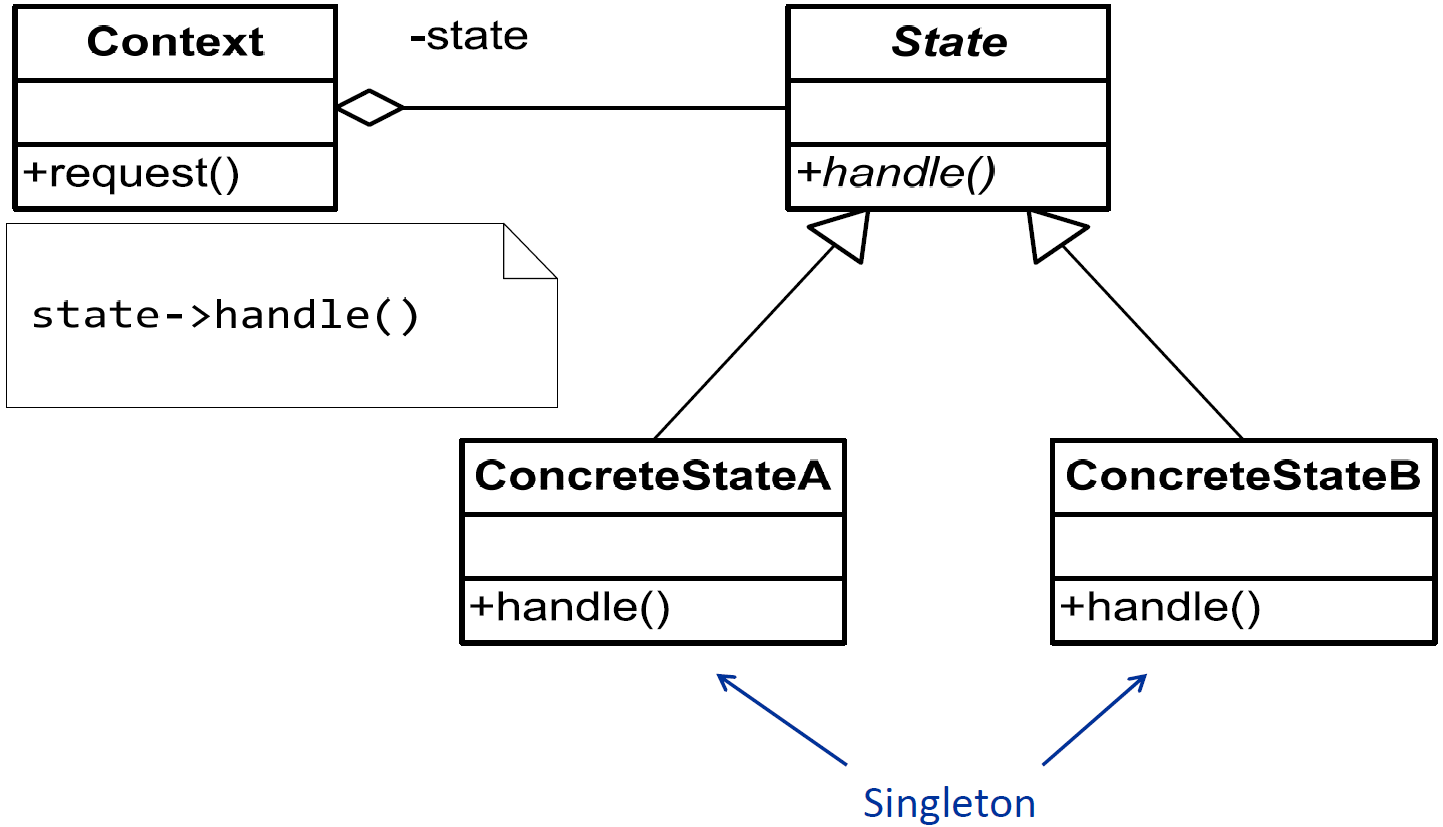
\includegraphics[width=0.7\columnwidth]{images/fsm_state_pattern_struktur.png}
\end{center}

%TODO: slides 4 + 6



\subsubsection{State-Event-Diagram -- Up/Down-Counter}
\label{State-Event-Diagram -- Up/Down-Counter - StatePattern}

\begin{center}
    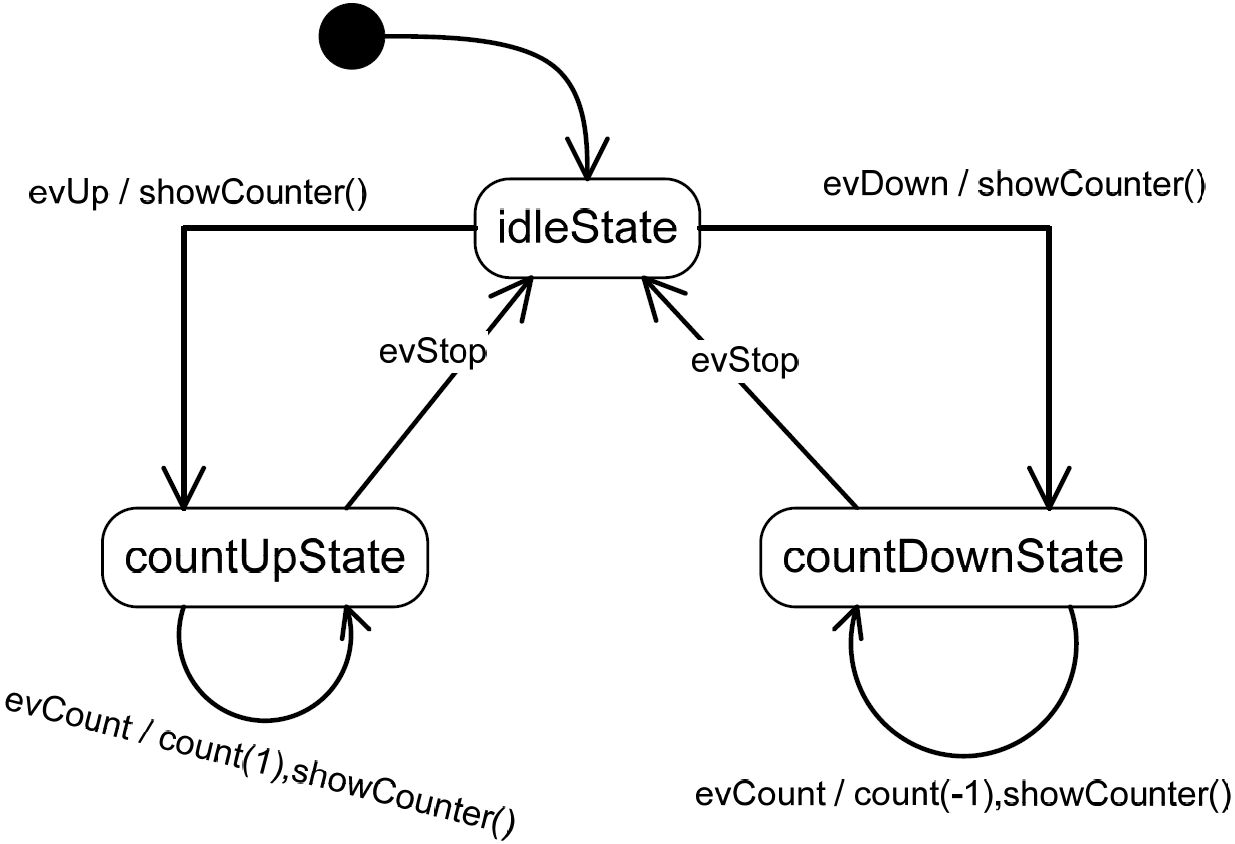
\includegraphics[width=0.7\columnwidth]{images/fsm_up-down-counter_diagramm_state_pattern.png}
\end{center}



\subsubsection{Implementation der Realisierung mittels StatePattern}

%TODO: describe stuff with StatePattern...
% \begin{outline}
%     \1 \textbf{Ereignisse (events)}
%         \2 Schnittstelle nach aussen \textrightarrow\ ändern Zustand der FSM
%         \2 Im \textbf{public} Teil der Klasse als enum definiert
%         \2 Keine Unitkürzel nötig
%     \1 \textbf{Zustände (states)}
%         \2 Im \textbf{private} Teil der Klasse als enum definiert \textrightarrow\ header-file
%     \1 \textbf{Aktueller Zustand} \mylstbox{currentState} wird in \textbf{privatem Attribut} von \mylstbox{CounterCtrl} gehalten
%     \1 Die FSM wird in \textbf{zwei Funktionen} implementiert
%         \2 Kontruktor (hier: \mylstbox{CounterCtrl::CounterCtrl(int initValue=0)})
%         \2 Prozess-Funktion (hier: \mylstbox{void CounterCtrl::process(CounterCtrl::Event e)}) \\
%             \textrightarrow\ Zustände prüfen, Zustandsübergänge veranlassen
%     \1 Anstossen einer FSM
%         \2 Initialisierung in \lstinline|main|-Funktion
%         \2 Überprüfung, welches Event aufgetreten ist meist in \mylstbox{do-while}-Schleife
% \end{outline}


\example{Up/Down-Counter (StatePattern, ohne actions)}

\para{Schnittstelle und Implementation von Counter}
Die Schnittstelle \mylstbox{counter.h} und die Implementation \mylstbox{counter.cpp} ändern sich nicht! \\
\textrightarrow\ Code-Beispiele siehe \ref{Realisieurng mit Steuerkonstrukt (objektorientiert in CPP)}


\para{Schnittstelle zur FSM} 
\lstinputlisting{snippets/fsm_state_pattern_CPP/fsm_CounterCtrl_state_pattern.h} 

\para{Implementation der FSM} 
\lstinputlisting{snippets/fsm_state_pattern_CPP/fsm_CounterCtrl_state_pattern.cpp} 


% \para{Schnittstelle abstrakte \lstinline|State|-Basisklasse}
% \lstinputlisting{snippets/fsm_state_pattern_CPP/fsm_CounterState_state_pattern.h} 


% \para{Implementation abstrakte \lstinline|State|-Basisklasse}
% \lstinputlisting{snippets/fsm_state_pattern_CPP/fsm_CounterState_state_pattern.cpp} 

        % \section{Modularisierung}

Ziel der Modularisierung ist eine \textbf{Reduktion der Komplexität.}
$$ \sum_{i} \text{complexity(problem)}_i < \text{complexity} \Big( \sum_{i} \text{problem}_i \Big) $$

\vspace{-0.2cm}


\subsection{Grundprinzip Modularisierung}

\begin{outline}
    \1 \textbf{Problem in (einfachere) Unterprobleme aufteilen} und diese Unterprobleme jeweils \textbf{einzeln angehen}
    \1 Abstraktion 
\end{outline}


\subsubsection{Motivation für Modularisierung}

\begin{outline}
    \1 \textbf{Grosse Projekte -- 'richtige' Softwaresysteme}
        \2 Systematischer Designansatz und strukturierter Aufbau ermöglichen effiziente \textbf{Arbeit im Team}
        \2 Schnittstellen müssen klar definiert werden
    \1 \textbf{Informatin Hiding}
        \2 Für die Nutzung eines Moduls (Unit) muss es gnügen, \textbf{nur die Schnittstellen} zu kennen
\end{outline}


\subsubsection{Phasenunterteilung beim Entwurf}

\begin{outline}
    \1 \textbf{Grobentwurf, Architektur (architectural design)}
        \2 (Software-) System im Grossen
        \2 Schnittstellen zu anderen (Nicht-Software-) Systemen
        \2 Datenstruktur im Grossen
        \2 \textbf{Aufteilung in Subsysteme}
        \2 \textbf{Schnittstellen zwischen Subsystemen}
    \1 \textbf{Feinentwurf}
        \2 Innenleben und Datenstruktur im Kleinen
\end{outline}


\subsection{Bewertung einer Zerlegung}

\begin{outline}
    \1 \textbf{Kopplung (coupling)}
        \2 Mass für Komplexität der Schnittstelle
    \1 \textbf{Kohäsion (cohesion)}
        \2 Aussage, wie stark eine funktionale Einheit wirklich zusammengehört
        \2 Mass die die Stärke des inneren Zusammenhangs
\end{outline}

\vspace{0.1cm}

\textbf{ \textrightarrow\ Ziel ist eine schwache Kopplung mit starker Köhäsion!}


\subsection{Kopplung}

\vspace{-0.2cm}

\begin{tikzpicture}[baseline=(current bounding box.north), >=latex]
    \node[anchor=north west] (kopplung) {
        \begin{minipage}{0.8\columnwidth}
            \begin{outline}
                \1 \textbf{Keine direkte Kopplung}
                \1 \textbf{Datenkopplung}
                    \2 Kommunikation ausschliesslich über Parameter
                \1 \textbf{Datenbereichskopplung}
                    \2 Ein Modul hat Zugriff auf eine Datenstruktur eines anderen Moduls. Es werden allerdings nur einzelne
                        Komponenten wirklich benötigt.
                \1 \textbf{Steuerflusskopplung} (control flow)
                    \2 Ein Modul beeinflusst Steuerfluss eines anderen Moduls
                \1 \textbf{Globale Kopplung}
                    \2 Kommunikation über globale Variablen, jedes Modul hat Zugriff
                \1 \textbf{Inhaltskopplung (Todsünde!)}
                    \2 Aus einem Modul heraus werden lokale Daten eines anderen Moduls modifiziert, obwohl dieses Modul
                        gar nicht vom anderen Modul aufgerufen wird.
            \end{outline}
        \end{minipage}
    };

    % Vertical arrow
    \draw[->, thick] ([xshift=-1em]kopplung.south west) -- ([xshift=-1em]kopplung.north west)
        node[very near start, left, color=red, thick]   {\shortstack{ \textbf{stark} \\ \textbf{(schlecht)}} }
        node[very near end, left, color=green]          {\shortstack{ \textbf{schwach} \\ \textbf{(gut)}} };
\end{tikzpicture}


\subsection{Kohäsion}

\vspace{-0.2cm}

\begin{tikzpicture}[baseline=(current bounding box.north), >=latex]
    \node[anchor=north west] (cohesion) {
        \begin{minipage}{0.8\columnwidth}
            \begin{outline}
                \1 \textbf{funktional}
                    \2 Die Teile einer Einheit bilden zusammen eine Funktion, bzw. eine Funktionsgruppe
                \1 \textbf{sequentiell}
                    \2 Teilfunktionen einer Einheit werden nacheinander ausgeführt, wobei das Resultat einer
                        Funktion als Eingabe für die nächste verwendet wird
                \1 \textbf{kommunikativ}
                    \2 Die Teilfunktionen einer Einheit werden auf den gleichen Daten ausgeführt, Reihenfolge
                        spielt keine Rolle
                \1 \textbf{prozedural}
                    \2 Teilfunktionen werden nacheinander ausgeführt, verknüpft über Steuerfluss
                \1 \textbf{\cbl{zeitlich}}
                    \2 Die Teile einer Einheit sind alle zu einer bestimmten Zeit auszuführen
                    \2 Typischer Fall: alle Initialisierungsfunktionen werden zusammengefasst
                \1 \textbf{logisch}
                    \2 (nicht zusammengehörende) Teilfunktionen einer Einheit gehören zu einer Einheit
                \1 \textbf{zufällig}
                    \2 Die Teilfunktionen einer Einheit haben keinen sinnvollen Zusammenhang
            \end{outline}
        \end{minipage}
    };

    % Vertical arrow
    \draw[->, thick] ([xshift=-1em]cohesion.south west) -- ([xshift=-1em]cohesion.north west)
        node[very near start, left, color=red, thick]   {\shortstack{ \textbf{schwach} \\ \textbf{(schlecht)}} }
        node[very near end, left, color=green]          {\shortstack{ \textbf{stark} \\ \textbf{(gut)}} };
\end{tikzpicture}


\subsubsection{Ziele bezüglich Kohäsion}

\begin{outline}
    \1 Kohäsion soll maximiert werden \\
        \textbf{ \textrightarrow\ starke Kohäsion führt automatisch zu schwacher Kopplung!}
    \1 Den genauen Wert der Kohäsion zu ermitteln ist \textbf{kein} Ziel
\end{outline}

\vspace{0.1cm}

\textbf{ \textrightarrow\ Zusammengehörendes zusammennehmen!}

% \columnbreak

\subsection{Guidelines -- gute Modularisierung}

\begin{outline}
    \1 \textbf{Zusammengehörendes zusammennehmen}
        \2 Defines für spezigisches Modul in Header-File des Moduls
    \1 Passende / aussagekräftige Namen für Variablen
    \1 'Interne' (private) Funktionen in \mylstbox{.c}-file deklarieren und definieren
    \1 Schnittstellenbeschreibung in Header-Dateien
        \2 Falls möglich: Doxygen verwenden
    \1 Lokale Funktionen (z.B. in \mylstbox{main.c}) bei Funktionsdeklarationen kommentieren
    \1 Allenfalls 'globalen' Header für Typdefinitionen
        \2 besser: Typen aus \mylstbox{stdint.h} verwenden
    \1 \mylstbox{uint8_t} etc. verwenden, wenn gezielt ein 8 Bit register angesprochen wird (und nur dann!)
    \1 Keine \mylstbox{initialization.h} Dateien \textrightarrow\ zeitliche Kohäsion!
        \2 generell keine Dateien wie: \mylstbox{global.h}, \mylstbox{defines.h}, \mylstbox{util.h}, \mylstbox{project.h}
\end{outline}

\vspace{0.2cm}

\textbf{Hinweis:} Für die Zurechtfindung in einem bestehenden Projekt müssen generell immer zuerst die \textbf{Header-Files studiert werden!}


\example{Schlechte vs. gute Modularisierung}

\begin{minipage}[t]{0.48\columnwidth}
    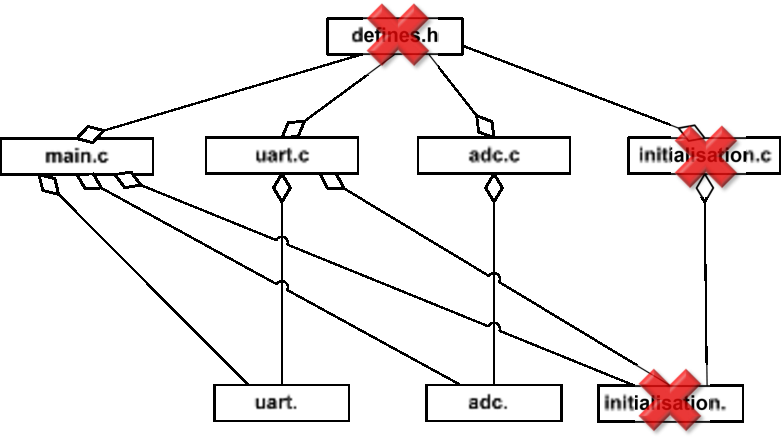
\includegraphics[width=\columnwidth, align=t]{images/modulaisierung_bsp_schlecht.pdf}
\end{minipage}
\hfill
\begin{minipage}[t]{0.48\columnwidth}
    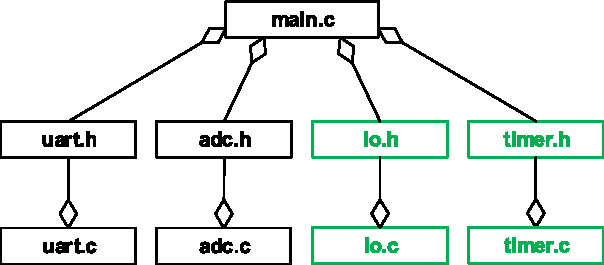
\includegraphics[width=\columnwidth, align=t]{images/modulaisierung_bsp_gut.pdf}
\end{minipage}

\vspace{-0.2cm}


\subsection{Package-Diagramm}

\begin{outline}
    \1 Ein Package besteht aus mindestens einer, üblich aus mehreren Klassen, die zusammengehören (Stichwort: \textbf{Kohäsion})
    \1 Im Package-Diagramm kann dargestellt werden, welche Packages mit welchen anderen Packages Verbindungen haben (dürfen) 
        \2 \textbf{Abhängigkeiten zwischen Packages} können sichtbar gemacht werden
    \1 Packagekonzept in C++: Namespaces umgesetzt
        \2 ein Namespace entspricht einem Package
\end{outline}


\example{Schlechtes vs. gutes Packaging}

\begin{center}
    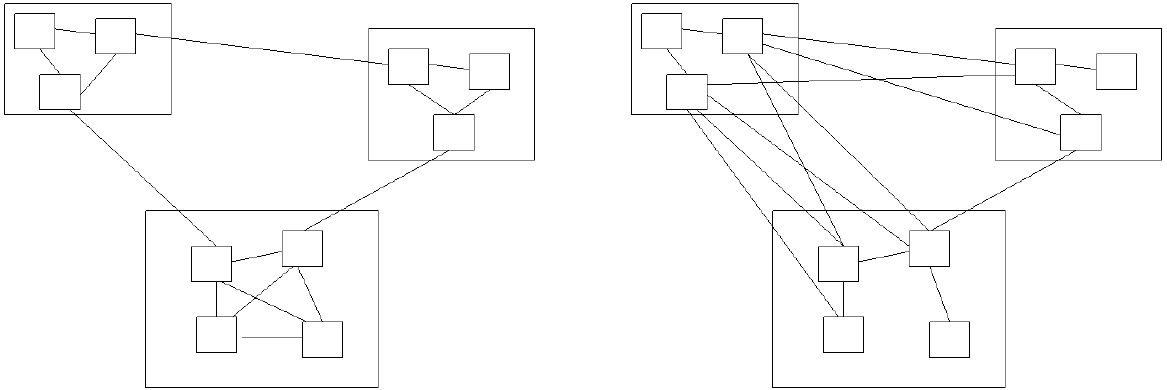
\includegraphics[width=0.9\columnwidth]{images/modulaisierung_bsp.png}
\end{center}

\vspace{-0.2cm}

links: hohe Kohäsion, tiefe Kopplung \textrightarrow\ gut \\
rechts: tiefe Kohäsion, hohe Kopplung \textrightarrow\ schlecht


        % % Embedded Software Patterns
        % \section{Patterns (Lösungsmuster)}

\textbf{Ein Software Pattern ist eine bekannte Lösung für eine Klasse von Problemen.}

\vspace{0.1cm}

\begin{minipage}[t]{0.48\columnwidth}
    \raggedright

    \begin{itemize}
        \item[+] Rad muss nicht immer neu erfunden werden 
        \item[+] Getestete / funktionierende Lösungen 
    \end{itemize}
\end{minipage}
\hfill
\begin{minipage}[t]{0.48\columnwidth}
    \raggedright

    \begin{itemize}
        \item[-] Wichtige Patterns müssen bekannt sein
        \item[-] Problemstellungen müssen als solche erkannt werden 
    \end{itemize}
\end{minipage}


\subsection{Arten von Patterns}

\begin{outline}
    \1 \textbf{Architekturmuster (Architectural Pattern)}
        \2 Legt die grundlegende Organisation einer Anwendung und die Interaktion zwischen den Komponenten fest
    \1 \textbf{Entwurfsmuster (Design Pattern)}
        \2 Die ursprüngliche Form des Pattern‐Ansatzes
    \1 \textbf{Implementationsmuster (Implementation Pattern)}
        \2 Behandelt grundsätzliche Implementationen immer wiederkehrender Codefragmente
\end{outline}


\subsection{Wichtige Patterns für Embedded Systems}

\subsubsection{Bereits bekannte Patterns}

\begin{minipage}[t]{0.48\columnwidth}
    \raggedright

    \begin{outline}
        \1 \textbf{FSM Implementationen}
            \2 State Pattern
            \2 Singleton Pattern
            \2 (Steuerkonstrukt mit switch-case)
            \2 (Tabellenvariante)
    \end{outline}
\end{minipage}
\hfill
\begin{minipage}[t]{0.5\columnwidth}
    \raggedright
    
    \begin{outline}
        \1 \textbf{'Mini-Patterns'}
            \2 Setzen / Löschen einzelner Bits
            \2 Behandlung asynchroner Ereignisse
                \3 Interrupts
                \3 Polling
    \end{outline}
\end{minipage}


\subsubsection{Creational Patterns}

Creational Patterns behandeln die \textbf{Erzeugung (und Vernichtung) von Objekten.}

\vspace{0.1cm}

% \begin{minipage}[t]{0.48\columnwidth}
%     \raggedright

%     \begin{outline}
%         \1 \textbf{Factory (Dependency injection)}
%             \2 Definition einer Schnittstelle zur Erzeugung eines Objekts, statt der direkten Erzeugung auf der Client-Seite
%         \1 \textbf{Singleton}
%             \2 stellt sicher, dass eine Klasse nur \textbf{ein einziges Objekt} besitzt
%     \end{outline}
% \end{minipage}
% \hfill
% \begin{minipage}[t]{0.5\columnwidth}
%     \raggedright
    
%     \begin{outline}
%         \1 \textbf{RAII (Resource Acquisition Is Initialization)}
%             \2 Die Belegung und Freigabe einer Ressource wird an die Lebensdauer eines Objektes gebunden. Dadurch wird eine
%                 Ressource z.B. 'automatisch' freigegeben.
%     \end{outline}
% \end{minipage}

\begin{outline}
    \1 \textbf{Factory (Dependency injection)}
        \2 Definition einer Schnittstelle zur Erzeugung eines Objekts, statt der direkten Erzeugung auf der Client-Seite
    \1 \textbf{Singleton}
        \2 stellt sicher, dass eine Klasse nur \textbf{ein einziges Objekt} besitzt
    \1 \textbf{RAII (Resource Acquisition Is Initialization)}
        \2 Die Belegung und Freigabe einer Ressource wird an die Lebensdauer eines Objektes gebunden. Dadurch wird eine Ressource 
            z.B. 'automatisch' freigegeben.
\end{outline}


\subsubsection{Structural Patterns}

Structural Patterns \textbf{vereinfachen Beziehungen} zu anderen Teilen.

\vspace{0.1cm}

% \begin{minipage}[t]{0.55\columnwidth}
%     \raggedright

%     \begin{outline}
%         \1 \textbf{Adapter (Wrapper, Translator, glue code)}
%             \2 Wandelt (adaptiert) eine Schnittstelle in eine für einen Client passendere Schnittstelle um
%         \1 \textbf{Facade}
%             \2 Bietet eine \textbf{einfache Schnittstelle} für die Nutzung einer meist viel \textbf{grösseren Library}
%     \end{outline}
% \end{minipage}
% \hfill
% \begin{minipage}[t]{0.43\columnwidth}
%     \raggedright
    
%     \begin{outline}
%         \1 \textbf{Proxy}
%             \2 'A proxy, in its most general form, is a class functioning as an interface to something else.'
%             \2 Oft ist es eine SW-Repräsentation eines HW-Teils, z.B. die Repräsentation einer Netzwerkverbindung
%     \end{outline}
% \end{minipage}

\begin{outline}
    \1 \textbf{Adapter (Wrapper, Translator, glue code)}
        \2 Wandelt (adaptiert) eine Schnittstelle in eine für einen Client passendere Schnittstelle um
    \1 \textbf{Facade}
        \2 Bietet eine \textbf{einfache Schnittstelle} für die Nutzung einer meist viel \textbf{grösseren Library}
    \1 \textbf{Proxy}
        \2 'A proxy, in its most general form, is a class functioning as an interface to something else.'
        \2 Oft ist es eine SW-Repräsentation eines HW-Teils, z.B. die Repräsentation einer Netzwerkverbindung
\end{outline}


\subsubsection{Behavioral Patterns}

Behavioral Patterns identifizieren \textbf{gemeinsame Kommunikationspatterns} zwischen Objekten und implementieren diese.

\vspace{0.1cm}

% \begin{minipage}[t]{0.48\columnwidth}
%     \raggedright

%     \begin{outline}
%         \1 \textbf{Mediator}
%             \2 definiert ein Objekt, welches das Zusammenspiel einer Menge von Objekten regelt
%             \2 ein Embedded System, das aus \textbf{mehreren Teilen} wie Sensoren und Aktoren besteht, wird \textbf{im Mediator
%                 softwaremässig zusammengebaut}
%     \end{outline}
% \end{minipage}
% \hfill
% \begin{minipage}[t]{0.48\columnwidth}
%     \raggedright
    
%     \begin{outline}
%         \1 \textbf{Observer (MVC)}
%             \2 Nicht nur bei Embedded Systems wichtig
%             \2 Wird als objektorientierte Variante präsentiert
%             \2 MVC-Prinzip kann auch prozedural mit Callbackfunktionen implementiert werden
%     \end{outline}
% \end{minipage}

\begin{outline}
    \1 \textbf{Mediator}
        \2 definiert ein Objekt, welches das Zusammenspiel einer Menge von Objekten regelt
        \2 ein Embedded System, das aus \textbf{mehreren Teilen} wie Sensoren und Aktoren besteht, wird \textbf{im Mediator
            softwaremässig zusammengebaut}
    \1 \textbf{Observer (MVC)}
        \2 Nicht nur bei Embedded Systems wichtig
        \2 Wird als objektorientierte Variante präsentiert
        \2 MVC-Prinzip kann auch prozedural mit Callbackfunktionen implementiert werden
\end{outline}

\vspace{0.1cm}

\textbf{Beispiel Mediator:} Bei einem Drucker mit mehreren Druckaufträgen von mehreren Personen teilt der Mediator die Aufträge jeweils korrekt


\subsubsection{Concurrency Patterns}

Concurrency Patterns kümmern sich um die \textbf{Ausführung in multi-threaded Umgebungen.}

\vspace{0.1cm}

% \begin{minipage}[t]{0.48\columnwidth}
%     \raggedright

%     \begin{outline}
%         \1 \textbf{Active Object}
%             \2 entkoppelt den Methodenaufruf von der Methodenausführung \\
%                 Methode soll sich nicht kümmern, in welchem Kontext sie aufgerufen wird
%     \end{outline}
% \end{minipage}
% \hfill
% \begin{minipage}[t]{0.48\columnwidth}
%     \raggedright
    
%     \begin{outline}
%         \1 \textbf{Lock}
%             \2 Synchronisationsprimitive, welche den unteilbaren Zugriff read-modify-write implementiert
%         \1 \textbf{Monitor}
%             \2 Monitor versteckt Synchronisationsanforderungen vor Client
%     \end{outline}
% \end{minipage}

\begin{outline}
    \1 \textbf{Active Object}
        \2 entkoppelt den Methodenaufruf von der Methodenausführung \\
            Methode soll sich nicht kümmern, in welchem Kontext sie aufgerufen wird
    \1 \textbf{Lock}
        \2 Synchronisationsprimitive, welche den unteilbaren Zugriff read-modify-write implementiert
    \1 \textbf{Monitor}
        \2 Monitor versteckt Synchronisationsanforderungen vor Client
\end{outline}


        % % Event-based Systems
        % \section{Event-based Systems}

\subsection{Ereignisse (Events)}

Reaktive Systeme reagieren auf (oft externe) Ereignisse (z.B. Digitale Inputs, Timer, Buttonclicks, etc.). Solche \textbf{Ereignisse sind per 
Definition asynchron und treten somit zu einem beliebigen Zeitpunkt auf.} 
Die Ereignisse können jedoch \textbf{synchron oder asynchron} umgesetzt werden.


\subsection{Synchrone Umsetzung von Ereignissen}

Ein '\textbf{normales' Programm} ist immer \textbf{synchron}. (Programm gibt vor, was wann ausgeführt wird.)

\subsubsection{Polling}

\begin{itemize}
    \item Programm fragt periodisch oder dauernd ab, ob irgendein Ereignis eingetreten ist
    \item Maximale Reaktionszeit wird durch Abfrageperiode und Anzahl Abfragen definiert (Looptime bei SPS)
    \item[+] Sehr einfach zu implementieren
    \item[-] Leerabfragen (Abfragen, bei welchen nichts eingetreten ist) können durch periodisches Abfragen (mittels Timer) reduziert, 
        aber nicht vermieden werden
\end{itemize}


\subsection{Asynchrone Umsetzung von Ereignissen}

Ziel der asynchronen Verarbeitung von Events ist es, dass die Prozessorzeit \textbf{genau dann und nur dann} beansprucht wird, wenn ein 
Ereignis eingetreten ist. \textrightarrow\ Interrupts


\subsection{Interrupt-Verarbeitung}

\begin{enumerate}
    \item I/O-Element generiert einen Interrupt Request
    \item Die CPU unterbricht das laufende Programm
    \item \textbf{Die Interrupts werden disabled (ausgeschaltet)}
    \item Das I/O-Element wird informiert, dieses deaktiviert den Interrupt Request
    \item Die Interrupt Service Routine (ISR) wird ausgeführt
    \item \textbf{Die Interrupts werden wieder enabled (eingeschaltet)}
    \item Die CPU führt das Programm an der unterbrochenen Stelle weiter
\end{enumerate}


\para{Sprungadresse nach Interrupt-Auslösung (ISR)}

\begin{outline}
    \1 \textbf{Non-vectored Interrupt (zentral)}
        \2 Alle Interrupts verzweigen zu einer \textbf{gemeinsamen Adresse}. Dort wird die Ursache bestimmt und zu einer
            spezifischen Behandlungsroutine verzweigt.
        \2[+] Nur eine zentrale Routine für die Behandlung notwendig
        \2[-] Information über die Ursache ist beim Eintreten bereits bekannt. Dann
                verzweigt man in die zentrale Routine, d.h. diese Information ist dann verloren. In der Routine muss diese
                Information wieder ermittelt werden.
    \1 \textbf{Vectored Interrupt (spezifisch)}
        \2 In einer Tabelle (\textbf{Interruptvektortabelle}, IVT) wird gespeichert, wohin bei welchem Interruptvektor
            verzweigt werden muss. \\
            \textrightarrow\ zu bevorzugende Methode!
\end{outline}


\subsection{Interruptvektortabelle (IVT)}

Für jeden Vektor muss eingetragen werden, welches die \textbf{Anfangsadresse} der Interrupt Service Routine
(ISR) ist, d.h. die \textbf{IVT ist nichts anderes als eine Tabelle (Array) von Funktionspointern.}

\vspace{0.1cm}

\textrightarrow\ Dieses Konzept kommt bei \textbf{allen asynchronen Mechanismen} zur Anwendung


\subsection{Model View Controller (MVC) aka Observer Pattern}

Ausgangslage: Daten (model) und verschiedene Darstellungsformen (views) der Daten (z.B. Balkendiagramm, Kuchendiagramm, Tabelle, etc.) \\
\textbf{\textrightarrow\ Die views sollen unbedingt vom model getrennt werden!}

\vspace{0.2cm}

Wie kann nun erreicht werden, dass bei \textbf{jeder Änderung} der Daten (model) alle Darstellungen aktualisiert werden? 
\textrightarrow\ Callback-Funktionen!


\subsection{Callback-Funktionen}

\begin{itemize}
    \item[+] Views werden \textbf{asynchron} genau informiert, wenn sich etwas im \textbf{model geändert} hat
    \item[+] An und für sich sind alle registrierten Funktionen nichts anderes als \textbf{Eventhandler eines bestimmten Events}
        \textrightarrow\ Darstellung (Definition der registrierten Funktionen) sauber von den Daten (model) \textbf{entkoppelt} 
\end{itemize}


\subsubsection{Callback-Funktionen in C}

Beim MVC gilt:

\vspace{0.1cm}

\begin{itemize}
    \item model wirkt als server
    \item views sind clients
\end{itemize}


\para{Event registieren (attach)}

\begin{outline}
    \1 Jeder client meldet beim server an, welche Ereignisse ihn interessieren
        \2 Anmeldung erfolgt über eine Funktion, welche der service anbietet
        \lstinputlisting[aboveskip=1mm, linewidth=\linewidth, morekeywords={[3], e, f}, firstnumber=1, firstline=1, lastline=3]{snippets/ebs_callback.c}
    \1 Der server trägt diesen \textbf{Funktionspointer} \mylstbox{f} in eine Tabelle ein und ruft \textbf{beim Eintreten des Ereignisses alle
        registrierten Funktionen} der Reihe nach je über den eingetragenen Funktionspointer auf
\end{outline}


\para{Event austragen (detach)}

\begin{outline}
    \1 Ein client kann sein Interesse an einem Ereignis beim Server auch wieder austragen
        \2 Der Server löscht dann den entsprechenden Eintrag (\textbf{Funktionspointer} \mylstbox{f}) wieder aus der Tabelle
        \lstinputlisting[aboveskip=1mm, linewidth=\linewidth, morekeywords={[3], e, f}, firstnumber=1, firstline=5, lastline=7]{snippets/ebs_callback.c}
\end{outline}


\subsection{Umsetzung der Callback-Funktionen in C (serverseitig)} 

\begin{outline}
    \1 Funktionspointer \mylstbox{foo_cbFunction} zu Callback-Funktionen definieren
        \lstinputlisting[aboveskip=1mm, linewidth=\linewidth, firstnumber=1, firstline=9, lastline=10]{snippets/ebs_callback.c}
    \1 Tabelle von Funktionspointern für jeden Event definieren und mit \textbf{Nullpointern initialisieren}
        \lstinputlisting[aboveskip=1mm, linewidth=\linewidth, morekeywords={[3], evNum, evClient}, firstnumber=1, firstline=12, lastline=13]{snippets/ebs_callback.c}
    \1 Aufruf der registrierten Clientfunktionen beim Eintreten des Events
        \lstinputlisting[aboveskip=1mm, linewidth=\linewidth, morekeywords={[3], evNum, i, evClient, client, arg}, firstnumber=1, firstline=15, lastline=24]{snippets/ebs_callback.c}
\end{outline}


\para{Mitteilung eines Events}

\vspace{0.1cm}

\begin{minipage}[t]{0.4\columnwidth}
    \raggedright
    Sobald (\textbf{asynchron}) ein Event eingetreten ist, kann dieser dem Server mit der Funktion
    \mylstbox[morekeywords={[3], e}]{void  foo_signalEvent(foo_Event e);} mitgeteilt werden.
\end{minipage}
\hfill
\begin{minipage}[t]{0.56\columnwidth}
    % CHECK: If there will be a full code example of callback functions, outcomment the following snippet
    \lstinputlisting[aboveskip=1mm, linewidth=\linewidth, morekeywords={[3], e, ev1Num, ev2Num, ev1Client, ev2Vlient}, firstnumber=1, firstline=26, lastline=42]{snippets/ebs_callback.c}
\end{minipage}


% Sobald (\textbf{asynchron}) ein Event eingetreten ist, kann dieser dem Server mit der Funktion
% \mylstbox[morekeywords={[3], e}]{void  foo_signalEvent(foo_Event e);} mitgeteilt werden.

% % CHECK: If there will be a full code example of callback functions, outcomment the following snippet
% \lstinputlisting[aboveskip=1mm, linewidth=\linewidth, morekeywords={[3], e, ev1Num, ev2Num, ev1Client, ev2Vlient}, firstnumber=1, firstline=26, lastline=42]{snippets/ebs_callback.c}


\subsection{Observer Pattern}

\subsubsection{Klassendiagramm (abstrakte Observer Basisklasse)}

\begin{center}
    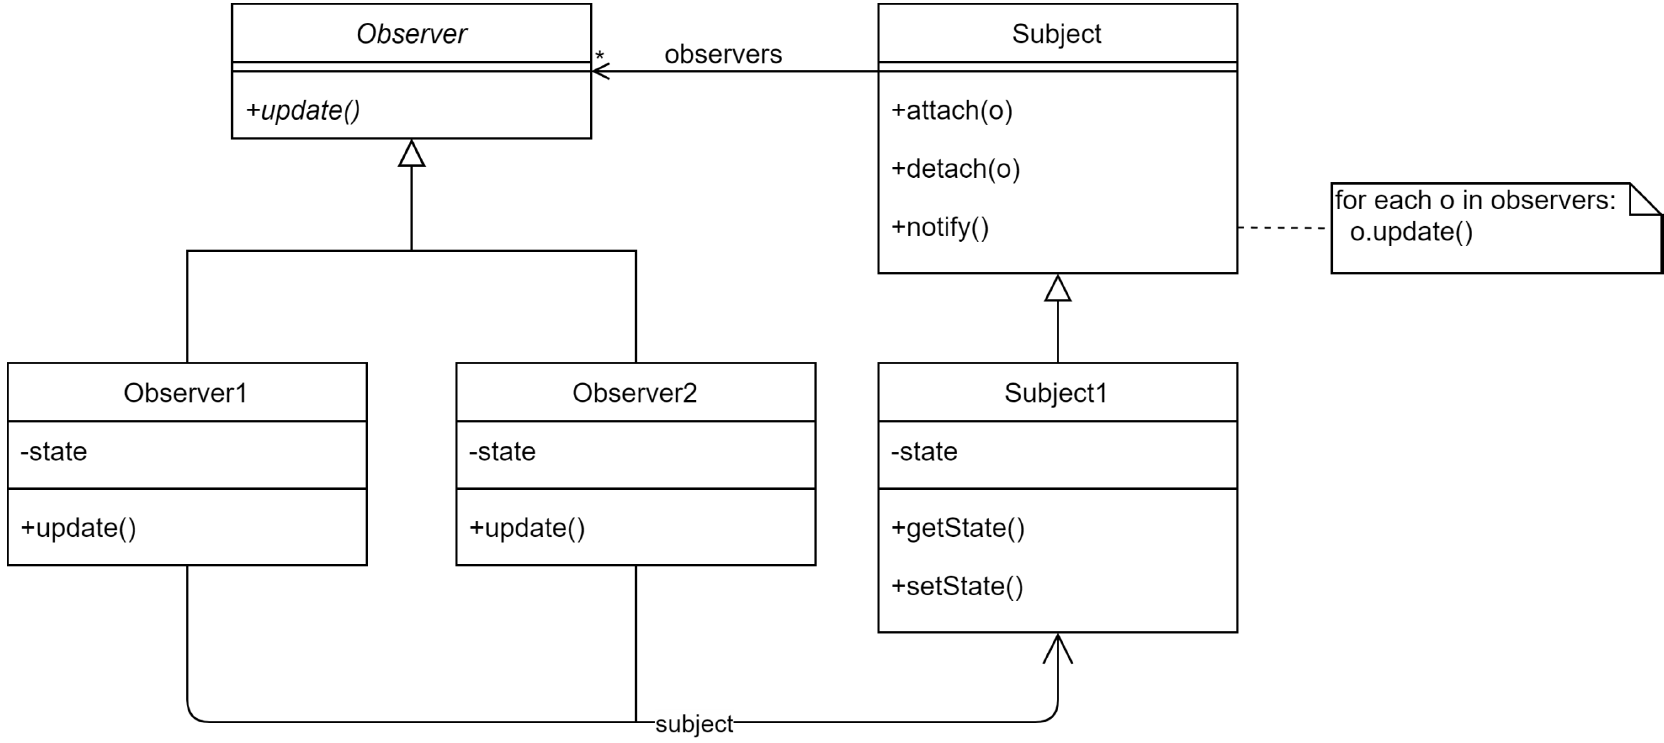
\includegraphics[width=0.8\columnwidth]{images/ebs_observer_pattern_klassendiagramm.png}
\end{center}


\subsubsection{Implementation in C++}

%TODO: write some stuff about how to implmenent that stuff
% slide 20 + eigene Erkenntnisse / Gedanken

\begin{outline}
    \1 \textbf{Observer-Klasse (abstrakte Basisklasse)}

    \1 \textbf{Observer-Subklassen}

    \1 \textbf{Subjekt Klasse}

    \1 \textbf{Subjekt1 Subklasse}
\end{outline}


\example{Observer Pattern in C++}

%TODO: code snippets
        % \section{Scheduling}
\label{Scheduling}

\subsection{Multitasking}

Mehrere (gleiche oder unterschiedliche) Tasks müssen erledigt werden. Dazu werden Ressourcen benötigt (z.B. \textbf{CPU}, Speicher, ...).
Wenn mehrere Tasks \textbf{dieselben Ressourcen} benötigen, nimmt der \textbf{Scheduler} die Zuteilung der Ressourcen an die einzelnen Tasks vor.

\vspace{0.1cm}

Bei der Zuteilung der Ressourcen wird darauf geachtet, dass alle \textbf{kritischen deadlines eingehalten} werden. \\
\textrightarrow\ Der Scheduler \textbf{priorisiert} also die \textbf{kritischen Tasks.} \\
Unter Umständen werden somit Deadlines von weniger kritischen Tasks verletzt.


\subsubsection{Zeitdefinitionen (Task)}

% NOTE: dieses Kapitel kommt auch schon in section 2 vor -> wurde aber wege Formatierung nicht verschoben sondern dupliziert
\begin{center}
    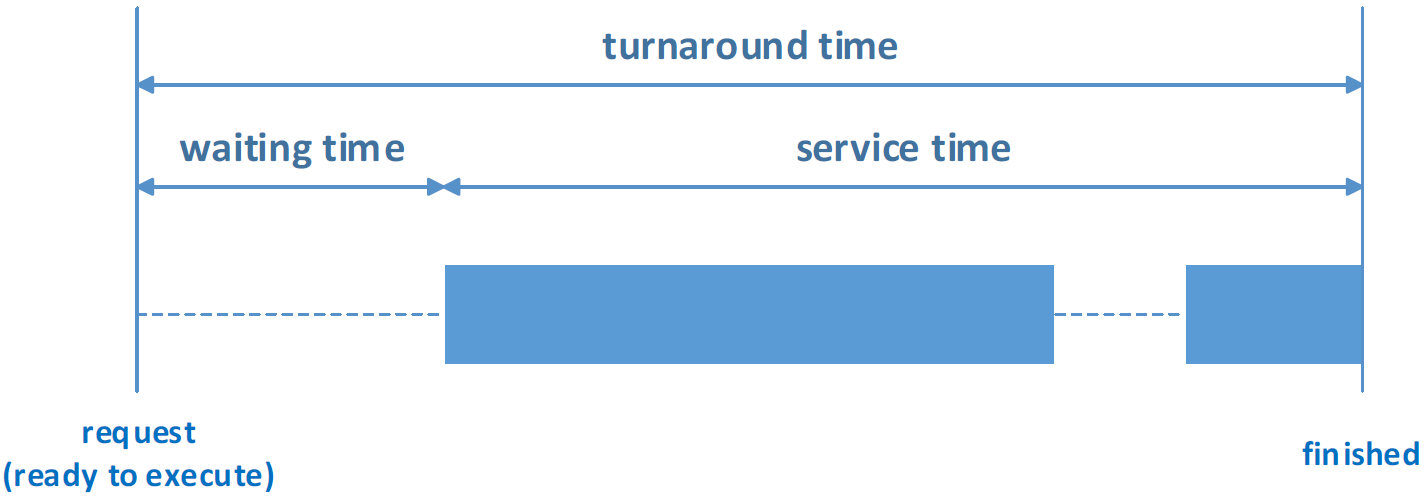
\includegraphics[width=0.7\columnwidth]{images/zeitdefinitionen_task.png}
\end{center}

\begin{outline}
    \1 \textbf{turnaround time:} (response time, Antwortzeit) 
        \2 Startet, wenn der Task bereit zur Ausführung ist und endet, wenn der Task fertig abgearbeitet ist
        \2 Zeit zwischen dem Vorhandensein von Eingangswerten an das System (Stimulus) bis zum Erscheinen der gewünschten Ausgangswerte.
    \1 \textbf{waiting time:} (Wartezeit)
        \2 Zeit zwischen Anliegen der Eingangswert und Beginn der Abarbeitung des Tasks
    \1 \textbf{service time:} (Bearbeitungszeit)
        \2 Zeit für Abarbeitung des Tasks \textrightarrow\ Unterbrechungen bzw. (preemptions) möglich 
\end{outline}


\subsubsection{Leistungsmerkmale}

\begin{minipage}[t]{0.52\columnwidth}
    \raggedright

    \begin{outline}
        \1 Durchsatz (throughput)
            \2 Anzahl erledigte Tasks pro Zeiteinheit
        \1 Mittlere Wartezeit (average waiting time)
    \end{outline}
\end{minipage}
\hfill
\begin{minipage}[t]{0.45\columnwidth}
    \raggedright

    \begin{outline}
        \1 Auslastung (utilization)
            \2 Prozentuale Auslastung einer Ressource
        \1 Weitere
    \end{outline}
\end{minipage}


\subsection{Scheduability}

Eine Menge von Tasks ist dann \textbf{scheduable}, wenn \textbf{alle Tasks zu allen Zeiten ihre deadlines einhalten} können. 
\textrightarrow\ Das ist immer das Ziel!

\subsubsection{Deadline -- Definition}

\begin{outline}
    \1 Spätestmöglicher Abschlusszeitpunkt (eines Tasks)
        \2 Bei periodischen Tasks ist dias meist gleichzeitig mit Beginn der nächsten Periode
\end{outline}


\subsection{Scheduling-Strategien}
\label{Scheduling-Strategien}

Folgende Algorithmen können dür die Zuteilung der Ressourcen (Scheduling) verwendet werden:

\begin{minipage}[t]{0.46\columnwidth}
    \raggedright

    \begin{outline}
        \1 \textbf{FCFS (First Come First Served)}
            \2 Einfachste Variante
        \1 \textbf{Round Robin}
            \2 Rund herum in fixer Reihenfolge
        \1 \textbf{Random}
    \end{outline}
\end{minipage}
\hfill
\begin{minipage}[t]{0.5\columnwidth}
    \raggedright

    \begin{outline}
        \1 \textbf{SJF (Shortest Job First)}
            \2[+] Mittlere Wartezeit minimal
            \2[-] längere Tasks können 'verhungern'
        \1 \textbf{Priority Scheduling}
            \2 unterbrechbar (preemptive) oder nicht unterbrechbar (non-preemptive)
            \2[-] tief priorisierte Taks können 'verhungern'
    \end{outline}
\end{minipage}

\vspace{0.1cm}

\textbf{Hinweis:} 'verhungern' heisst, dass ein Task gar keine Ressourcen erhält


\subsection{Cooperative Multitasking}

Kooperative Task-Zuteilung ist bei \textbf{fairen} Tasks möglich.

\vspace{0.1cm}

\begin{outline}
    \1 Aktiver Task entscheidet selbst, wann er CPU wieder für andere Tasks freigibt
        \2 Unfaire und abgestürzte Tasks blockiert andere Tasks
    \1 Nächster Task kann mit beliebigem Algorithmus ermittelt werden \\
        \textrightarrow\ siehe Abschnitt \ref{Scheduling-Strategien}
    \1 Sehr einfach zu implementieren
\end{outline}


\subsection{Preemptive Multitasking / Scheduling}
\label{Preemptive Multitasking / Scheduling}

Preemptive Multitasking wird meistens in RTOS verwendet. \\
\textbf{Der Task mit höchster Priorität wird immer ausgeführt.} Unter Umständen muss dabei ein Task mit niedrigerer Priorität
\textbf{unterbrochen} werden. 

\vspace{0.1 cm}

Es gibt zwei Arten von Preemptive Multitasking Algorithmen:

\begin{outline}
    \1 \textbf{dynamic-priority Algorithmen}
        \2 Prioritäten werden zur Laufzeit laufen angepasst (z.B. aufgrund von vorhandenen deadlines)
    \1 \textbf{static-priority Algorithmen}
        \2 Prioritäten werden zur Entwicklungszeit festgelegt und nicht geändert.
        \2 Einfacher als dynamic-priority Algorithmen!
\end{outline}


\subsection{Rate Monotonic Scheduling (RMS)}

RMS beschreibt Regel, bei deren Einhaltung eine Konfiguration \textbf{immer scheduable} ist.


\subsection{Rate Monotonic Scheduling Theorem}
\label{Rate Monotonic Scheduling Theorem}

\subsubsection{Zwingende Voraussetungen}

\begin{itemize}
    \item Perioische Tasks
    \item static priority preemptive scheduling \textrightarrow\ siehe Abschnitt \ref{Preemptive Multitasking / Scheduling}
\end{itemize}


\subsubsection{Regeln für optimales Scheduling}

Für jeden Task $T_i$ wird die Periode $p_i$ und die (worst case) execution time $e_i$ ermittelt, bzw. geschätzt. \\
Die Prioritäten mussen den Tasks zwingend folgendermassen zugewiesen werden:

\vspace{0.1cm}

\textbf{Tasks mit kürzerer Periode (d.h. mit hoher Rate) erhalten höhere Priorität (rate-monotonic)}


\subsubsection{Berechnung der Auslastung einer Ressource}

\begin{minipage}[t]{0.48\columnwidth}
    Jeder Task $T_i$ trägt mit der Teilauslastung $u_i = \frac{e_i}{p_i}$ zur Gesamtauslastung $U$ bei.
\end{minipage}
\hfill
\begin{minipage}[t]{0.48\columnwidth}
    \vspace{-0.2cm}
    $$ U = \sum\limits_{i} \frac{e_i}{p_i} $$
\end{minipage}


\subsection{Vorgehen -- Rate Monotonic Scheduling}

\begingroup
\renewcommand{\outlinei}{enumerate}
\renewcommand{\outlineii}{itemize}
\begin{outline}
    \1 Tasks priorisieren (Task mit kleinster Periode hat höchste Priorität!)
    \1 Task mit höchster Priorität aufzeichnen
    \1 Task mit zweithöchster Priorität 'regulär' zeichnen mit folgenden Sonderregelungen
        \2 Bei Bedarf warten (W), bis höher priorisierter Task abgeschlossen ist 
        \2 Höher priorisierte Tasks (bereits gezeichnet) unterbrechen (P) aktuellen Task
    \1 Punkt 3 wiederholen, bis alle Tasks aufgezeichnet sind und sich das Muster wiederholt
\end{outline}
\endgroup


\example{Rate Monotonic Scheduling}

\begin{minipage}[t]{0.55\columnwidth}
    Gemäss gegebener Tabelle sind die Tasks folgendermassen priorisiert:
    $$ T_1 > T_3 > T_2 $$
    In dieser Reihenfolge werden die Tasks aufgezeichnet!
\end{minipage}
\hfill
\begin{minipage}[t]{0.38\columnwidth}
    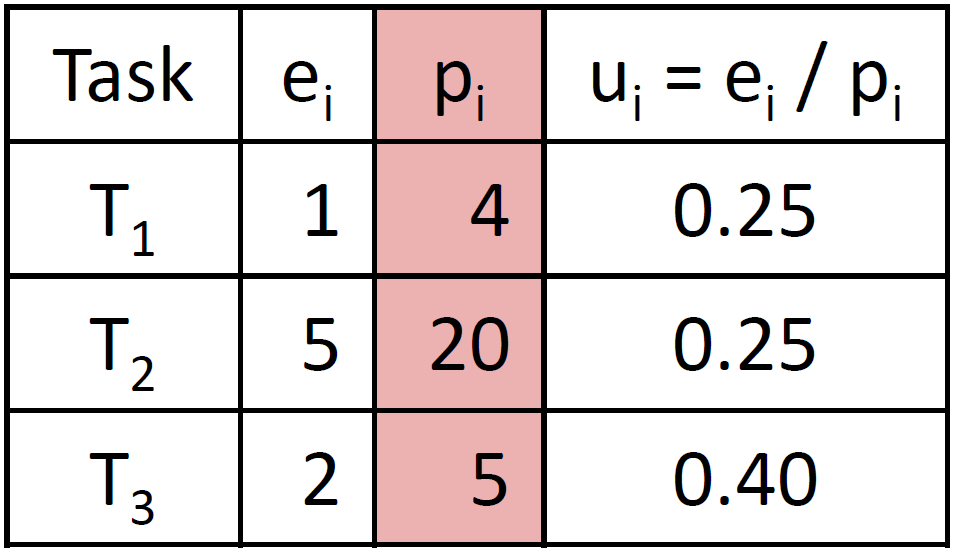
\includegraphics[width=\columnwidth, align=t]{images/scheduling_RMS_example_tabelle.png}
\end{minipage}

\begin{center}
    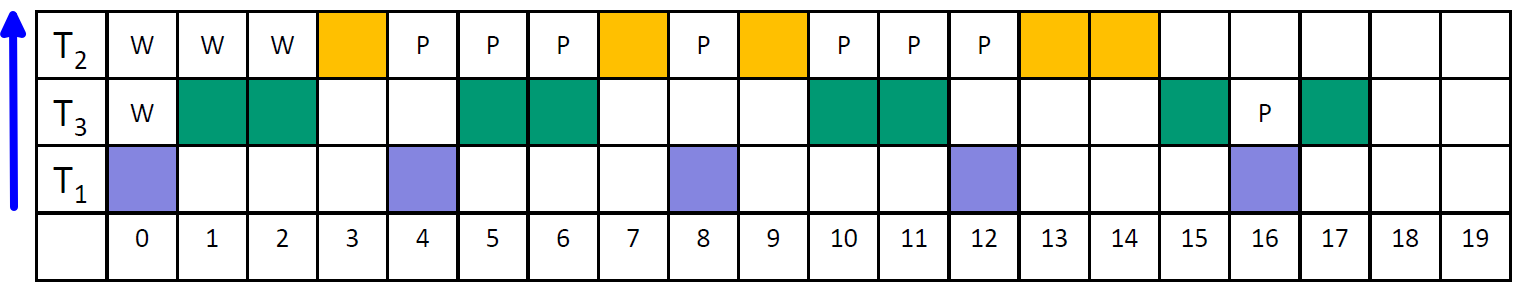
\includegraphics[width=\columnwidth]{images/scheduling_RMS_example_schedule.png}
\end{center}


\subsection{RMA Bound (RMA = Rate Monotonic Approach)}

Jede Konfiguration mit $n$ periodischen Tasks ist \textbf{immer} RM scheduable, wenn die Gesamtauslastung $U$ 
\textbf{unterhalb oder gleich} der RMA Bound $U(n)$ liegt

$$ \text{RMA-Bound} \qquad U(n) = n \cdot \big( 2^{\frac{1}{n}} - 1 \big)  $$

\begin{center}
    \begin{tabular}{l cccccc}
        \toprule
        $\bm{n}$                    & $2$       & $3$       & $4$       & $5$       & $10$      & $\infty$                      \\
        \midrule
        $\bm{U(n)}$ \textbf{in} \%  & $82.4$    & $78.0$    & $75.7$    & $74.4$    & $71.7$    & $\bm{\ln(2) \approx 69.3}$    \\
        \bottomrule
    \end{tabular}
\end{center}

\textrightarrow\ Liegt die Gesamtauslastung unter $69.3$ \%, ist die Konfiguration \textbf{immer} RM schedulable


\subsection{Anleitung für Zuweisung der Prioritäten bei RMS}

\begin{itemize}
    \item Prioritäten immer gemäss RMS zuweisen. (manuelle Zuweisung gibt keine bessere Lösung)
    \item Falls Auslastung nicht grösser als RMA Grenze, dann ist Konfiguration RM schedulable
    \item Falls Auslastung \textbf{grösser} ist, muss \textbf{manuell analysiert} werden, on Konfiguration schedulable ist
    \item 100 \% Auslastung könnte erreicht werden, wenn alle Perioden harmonisch sind, d.h. jede längere Periode ist ein exaktes
        Vielfaches aller Perioden kürzerer Dauer, \\
        z.B. (10, 20, 40, 80)
    \item Harmonische Perioden verringern die Unterbrechung (preemptions) von niedriger priorisierten Tasks \\
        \textrightarrow\ (10, 20, 40) ist gegenüber (10, 20, 50) zu bevorzugen, falls möglich
\end{itemize}


        % % Gleichzeitigkeit (Concurrency)
        % \section{Concurrency (Gleichzeitigkeit)}

Programme von praktischem Nutzen führen meist mehrere Arbeiten 'gleichzeitig' durch. Beispielsweise soll bei einem Embedded System ein Roboterarm 
bewegt werden, während 'gleichzeitig' mit einem übergeordneten System kommuniziert wird.


\subsection{Parallel Computing vs. Concurrent Computing}


\begin{outline}
    \1 \textbf{Parallel Computing}
        \2 Ausführung verschiedener Tasks \textbf{tatsächlich gleichzeitig}
        \2 Nicht möglich auf single-core System
    \1 \textbf{Concurrent Computing}
        \2 Ausführung verschiedener Tasks \textbf{wirkt nur gleichzeitig}
        \2 Verschiedene Tasks erhalten verschiedene 'time slices' \textrightarrow\ Ein Task pro time slice
        \2 Auf single- und multi-core Systemen möglich
\end{outline}


\subsection{Warum man Concurrency nicht verwenden sollte}

\begin{outline}
    \1 \textbf{Concurrency (mit Prozessen, Tasks, Threads) kostet immer}
        \2 Stack
        \2 Braucht context switch (Umschalten von einen zum anderen Prozess, Task, Thread) \\
            \textrightarrow\ Alter context (Registerwerte, Steck, etc.) muss gespeichert, neuer geladen werden 
        \2 Zugriff auf gemeinsame Ressourcen muss synchronisiert werden \\
            \textrightarrow\ fehleranfällig (wird vergessen / falsch gemacht)
    \1 \textbf{Komplexität steigt}
        \2 Sequenzielle Programme sind einfacher zu verstehen als parallele Programme
\end{outline}

\vspace{0.1cm}

\textbf{ \textrightarrow\ Concurrency nur dann einsetzen, wenn wirklich ein Nutzen vorhanden ist!}


\subsection{Synchronisation}

Wenn parallele Einheiten \textbf{gemeinsame Ressourcen} benützen, muss der Zugriff auf die Ressourcen geregelt (synchronisiert) werden.
Wenn dies nicht gemacht wird kann es sein, dass zwei Tasks dieselbe Ressource 'falsch' verwenden. \textrightarrow\ 'Deadlock'

\vspace{0.1cm}

\textbf{Achtung: } 'Ein Bisschen warten' ist \textbf{keine} Synchronisation!


        % POSIX-Programmierung
        \section{POSIX Threads Programming}

Für UNIX Systeme steht ein stardardisiertes threads programming interface in C zur Verfügung (POSIX threads / pthreads).


\subsection{UNIX Process vs. UNIX Thread}

\begin{center}
    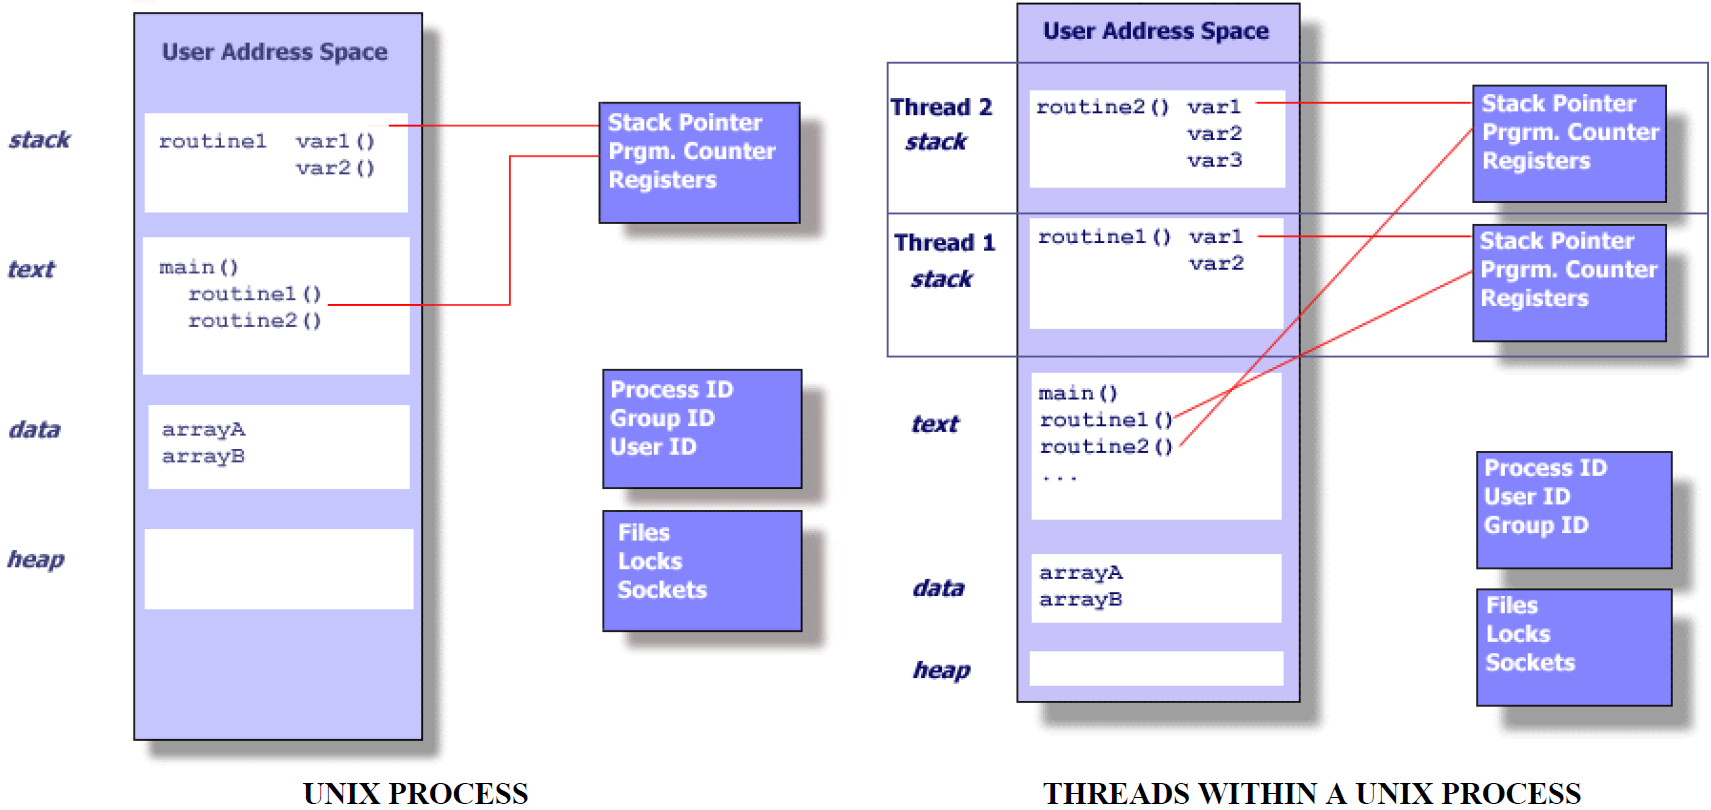
\includegraphics[width=0.75\columnwidth]{images/posix_process_threads.png}
\end{center}


\subsubsection{UNIX Process}

\begin{outline}
    \1 \textbf{heavyweight process} (generiert von Betriebssystem)
    \1 Prozess erfordert \textbf{erheblichen overhead}, da Informationen über Programmressourcen und 
        den Ausführungsstatus des Programms, beispielsweise:
        \2 Prozess-ID, Prozessgruppen-ID, Benutzer-ID und Gruppen-ID
        \2 Environment, Programmanweisungen
        \2 Register, Stack, Heap
        \2 Datei-Deskriptoren, Signal-Aktionen
        \2 Gemeinsame Bibliotheken
        \2 Werkzeuge für die prozessübergreifende Kommunikation
\end{outline}


\subsubsection{UNIX Thread}

\begin{outline}
    \1 lightweight 'process' (weniger overhead)
    \1 Unabhängiger 'stream of instructions', welcher simultan mit anderen 'streams of instructions' ablaufen kann %CHECK: german names...
    \1 Prozedur, welche unabhängig von ihrem (aufrufenden) main-Programm abläuft
    \1 \textbf{Threadsexistieren in einem Prozess und nutzen dessen Ressourcen}
        \2 Sobald ein Prozess ended, enden auch die darin existierenden Threads!
    \1 \textbf{Ein Thread benutzt den gleichen Adressraum wie andere Threads im gleichen Prozess}
        \2 Daten können einfach mit anderen Threads im gleichen Prozess geteilt werden
    \1 Threads werden vom Betriebssystem 'gescheduled'
    \1 Ein Thread dupliziert nur die essenziellen Ressourcen die er braucht, um unabhängig 'schedulable' zu sein:
        \2 Stack pointer, Register
        \2 Scheduling properties (policy / priority)
        \2 Set of pendding and blocked signals  % CHECK: in german...
        \2 Thread-spezifische Daten
\end{outline}

\vspace{0.1cm}

\textbf{ \textrightarrow\ Gleichzeitigkeit wird in der Programmierung mit Threads umgesetzt!}


\subsection{pthreads API}

\subsubsection{Includes / Compile \& Link}

\begin{outline}
    \1 \mylstbox{#include <pthread.h>} wird benötigt
    \1 Methoden der pthreads API starten mit \mylstbox{pthread_}
    \1 Source files, welche pthreads verwenden, sollen mit \mylstbox{-pthread} kompiliert werden
    \1 Für das file-linking muss der command \mylstbox{-lpthread} verwenet werden
\end{outline}


\example{Compiling / Linking file printer.c}

\begin{description}
    \item[Compiling:] \lstinline|clang -c -Wall -pthread printer.c|
    \item[Linking:]   \lstinline|clang -o printer printer.o -Wall -lpthread|
\end{description}


\subsubsection{Thread starten / beenden}

\begin{outline}
    \1 Jede Funktion mit der folgenden interface kann eine Thread-Methode werden
        \2 Als Parameter / Return-Wert sind alle Pointer-Datentypen möglich \\ %CHECK if this is correct...
        \mylstbox[aboveskip=1mm, linewidth=\linewidth, morekeywords={[3], arg}]{void* threadRoutine(void* arg);}
    \1 Ein Thread wird mit der folgenden Funktion gestartet:
        \lstinputlisting[aboveskip=1mm, linewidth=\linewidth, morekeywords={[3], thread, attr, arg}, morekeywords={[2], pthread_t, pthread_attr_t}]{snippets/posix_start_thread.c}
    \1 Ein Thread kann mit einer der folgenden drei Arten beendet werden
        \2 Thread ruft Funktion \mylstbox[aboveskip=1mm]{pthread_exit()} auf
        \2 Thread springt aus Thread Routine \mylstbox[aboveskip=1mm]{startRoutine} zurück
        \2 Thread wird mit Funktion \mylstbox[aboveskip=1mm]{pthread_cancel()} abgebrochen
\end{outline}


\subsubsection{Warten, bis ein Thread beendet ist}

\begin{outline}
    \1 Nach dem Starten des Threads bzw. am Ende des main-Programms kann eine Endlos-Schleife eingefügt werden
        \2 \textbf{Dies sollte nie gemacht werden}, da der Prozess so die gesamten CPU-Ressourcen braucht
    \1 Entsprechende Funktion aus pthreads API verwenden
        \lstinputlisting[aboveskip=1mm, linewidth=\linewidth, morekeywords={[3], thread, attr}, morekeywords={[2], pthread_t, pthread_attr_t}]{snippets/posix_wait_for_thread_termination.c}
\end{outline}


\subsection{Beispiel: thread API}

% \begin{center}
%     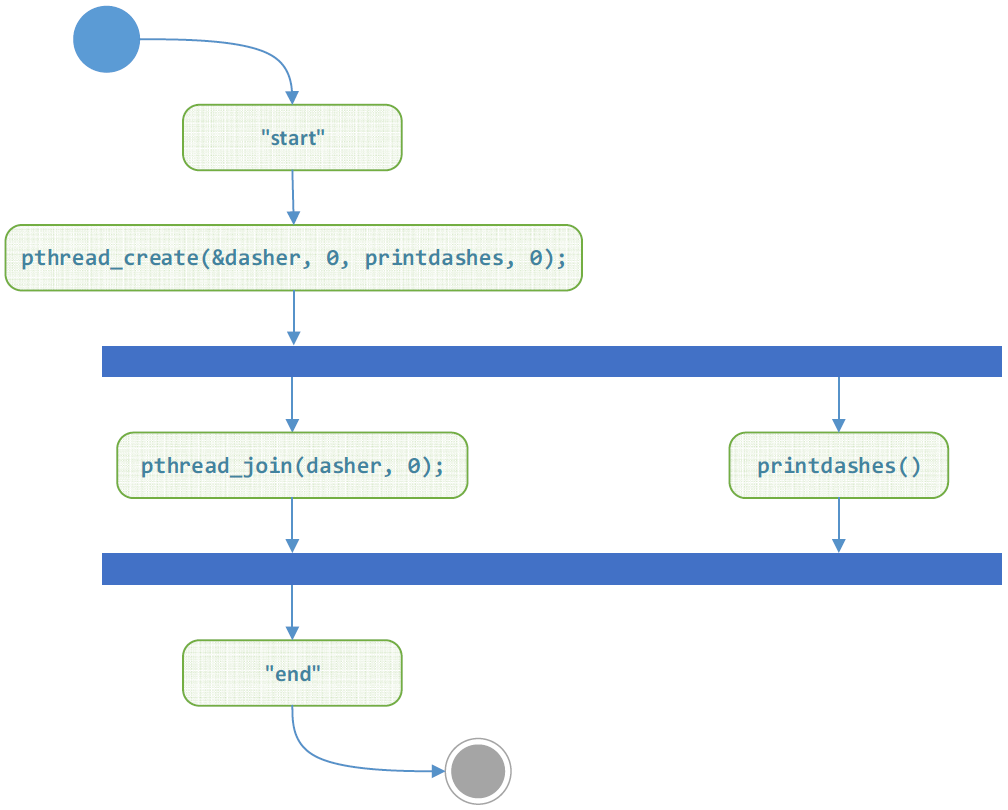
\includegraphics[width=0.8\columnwidth]{images/posix_thread_fork_join.png}
% \end{center}
\begin{minipage}[t]{0.48\columnwidth}
    \lstinputlisting[aboveskip=1mm, firstnumber=1, firstline=1, lastline=23, morekeywords={[3], arg, ret, dasher, i}, morekeywords={[2], pthread_t}]{snippets/posix_join.c}
\end{minipage}
\hfill
\begin{minipage}[t]{0.48\columnwidth}
    \lstinputlisting[aboveskip=1mm, firstnumber=24, firstline=24, lastline=48, morekeywords={[3], arg, ret, dasher, i}, morekeywords={[2], pthread_t}]{snippets/posix_join.c}
\end{minipage}


\subsection{Thread-safeness}
Thread-safeness bezieht sich auf die Fähigkeit einer Anwendung, mehrere Threads gleichzeitig auszuführen,
\textbf{ohne 'clubbering' und 'race conditions'} zu verursachen. Damit Thread-safeness gewährleistet werden kann, ist \textbf{Synchronisation}
erforderlich.

\begin{description}
    \item[clubbering:] Speicher durcheinander bringen, wenn mehrere Threads den gleichen Speicher benötigen und 'falsch' darauf zugreifen
    \item[race conditions:] Programmablauf und Endergebnis hängen davon ab, in welcher Reihenfolge 'gleichzeitig' ablaufende Threads auf z.B. eine
        globale Variable im Speicher zufreifen und das Verhalten somit unvorhersehbar wird
\end{description}


\subsubsection{Empfehlung: Thread-Safeness}

Wenn Thread-safeness nicht explizit garantiert ist (z.B. von einer Library, welche verwendet wird), muss  angenommen werden, dass sie 
\textbf{nicht thread-safe} ist! \\
Um in einem solchen Fall Thread-safeness zu gewährleisten, können die Aufrufe einer 'unsicheren' Funktion \textbf{serialisiert} werden.


\subsection{Quasi-Parallelität / 'Prozess'-Zustände}

\subsubsection{Prozess-Zustände}

\begin{minipage}[t]{0.45\columnwidth}
    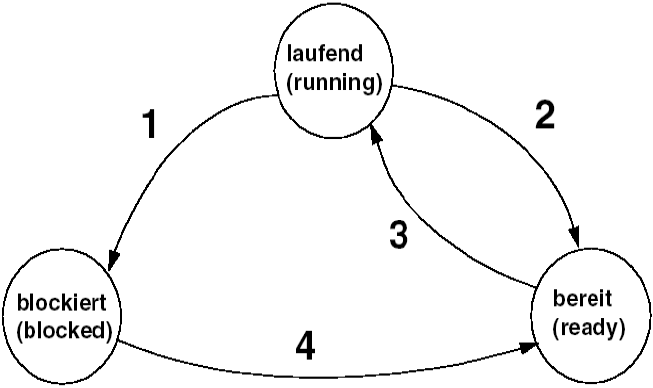
\includegraphics[width=\columnwidth, align=t]{images/posix_process_states.png}
\end{minipage}
\hfill
\begin{minipage}[t]{0.5\columnwidth}
    \begin{enumerate}
        \item I/O Operation, Warten auf Bedingung
        \item Scheduler entzieht CPU
        \item Scheduler weist CPU zu
        \item I/O beendet, Bedigung erfüllt
    \end{enumerate}
\end{minipage}

\vspace{0.2cm}

\begin{minipage}[t]{0.4\columnwidth}
    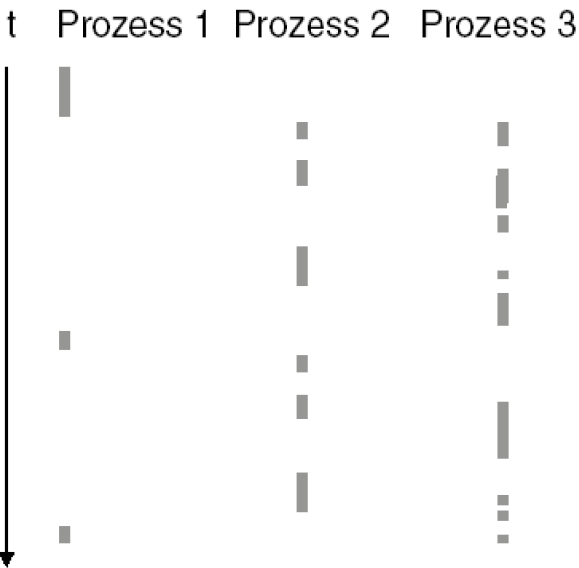
\includegraphics[width=\columnwidth, align=t]{images/concurrency_quasi_parallelitaet.png}
\end{minipage}
\hfill
\begin{minipage}[t]{0.58\columnwidth}
    \raggedright
    \begin{outline}
        \1 Prozesse / Threads warten die 'meiste Zeit' \\
            \textrightarrow\ blocked (z.B. \mylstbox{join} blockiert andere Threads)
        \1 Scheduler ordnet CPU denjenigen Prozess / Thread zu, die im Zustand 'ready' sind und 'etwas zu tun haben'
        \1 Die Zuordnung hängt vom verwendeten Scheduling-Algorithmus ab:
            \2 First come First serve Scheduling: Eine Queue mit allen Prozessen, wobei nächster Prozess jeweils hinten angehängt wird und erster 
                Eintrag der Queue aktuell ausgeführt wird
            \2 Priority Scheduling: Pro Priorität gibt es eine Queue. Abarbeitung je nach Algorithmus anders
    \end{outline}
\end{minipage}


% -------------------------------------------------------------------------------------------------------------------------------------------------
% CHECK: new section?
\subsection{Synchronisation}

Synchronisation wird benötigt, um den \textbf{Zugriff auf gemeinsame Ressourcen} in Critical Sections (CS) zu 'kontrollieren'.


\subsubsection{Defintition: Critical Section (CS)}

\begin{outline}
    \1 Codebereich, in dem nebenläufige oder parallele Prozesse auf gemeinsame Ressourcen zugreifen
        \2 Zu jeder Zeit darf sich \textbf{höchstenns ein Prozess} im kritischen Abschnitt befinden
    \1 Der Exklusive Zugriff durch höchstens einen Prozess wird mittels \textbf{gegenseitigem Ausschluss (Mutex)} sichergestellt
        \textrightarrow\ Siehe Abschnitt \ref{Mutex (mutual exclusion)}
\end{outline}


\subsubsection{Forderungen an die Synchronisation}

\begin{enumerate}
    \item Maximal ein Prozess in einem kritischen Abschnitt (CS)
    \item Über Abarbeitungsgeschwindigkeit, bzw. Anzahl Prozesse dürfen keine Annahmen getroffen werden
    \item Kein Prozess darf \textbf{ausserhalb} eines kritischen Abschnitts einen anderen blockieren
    \item Jeder Prozess, der am Eingang eines kritischen Abshcnitts wartet, muss irgendwann den Abschnitt betreten dürfen 
        (\textbf{fairness condition}) \textrightarrow\ Verhinderung von 'starvation'
\end{enumerate}


% CHECK: new section?
\subsection{Mutex (mutual exclusion)}
\label{Mutex (mutual exclusion)}

Die Lösungsstruktur 'Mutex' (gegenseitiger Ausschluss) stellt sicher, dass höchstens ein Prozess auf eine Critical Section (CS) zugreift. 


\subsubsection{Mutex -- Ablauf}

\begin{minipage}[c]{0.62\columnwidth}
    \raggedright

    \begin{description}
        \setlength\itemsep{2em}
        \item[Zugriffsprüfung:] Warten bis der Zugang frei wird
        \item[Sperren:] Signal wird für andere auf Rot gesetzt, damit nur ein Prozess im kritischen Abschnitt sein kann
        \item[Freigeben:] Rotes Signal wird wieder gelöscht
    \end{description}
\end{minipage}
\hfill
\begin{minipage}[c]{0.37\columnwidth}
    \begin{center}
    \begin{tikzpicture}
        [
            %transform canvas={scale=1.0},
            scale = 0.7,
            >=latex,
            bluebox/.style={rectangle, draw=black, fill=blue!40, thick, minimum width=1.5cm, minimum height=0.6cm, align=center},
            redbox/.style={rectangle, draw=black, fill=redcontrast!70, text=white, thick, minimum width=1.5cm, minimum height=0.6cm, align=center},
        ]
        % define styles
        
        % nodes
        \node[bluebox]      (Zugriff)                                               {Zugriff\\erlaubt?};
        \node[bluebox]      (Sperren)           [below= 0.4cm of Zugriff]           {Sperren};   
        \node[redbox]       (CS)                [below= 0.3cm of Sperren]           {kritischer\\Abschnitt};
        \node[bluebox]      (Freigeben)         [below= 0.3cm of CS]                {Freigeben};
        
        \node               (wait)              [right= 0.2cm of Sperren]           {\lstinline|waitFor(signal)|};
        \node               (send)              [right= 0.2cm of Freigeben]         {\lstinline|send(signal)|};
        
        % arrows between nodes
        \draw[->, thick] (Zugriff.south)    to (Sperren.north);
        \draw[->, thick] (Sperren.south)    to (CS.north);
        \draw[->, thick] (CS.south)         to (Freigeben.north);
    \end{tikzpicture}
\end{center}
\end{minipage}


\subsubsection{Verwendung von Signalen und Semaphoren}

\begin{outline}
    \1 Jeder Prozess wartet vor dem Betreten der CS auf ein gemeinsames Signal
        \2 Wenn das Signal gesetzt ist, ist CS frei
        \2 Mehrere Prozesse können gleichzeitig warten \textrightarrow\ Schedulingalgorithmus bestimmt 'nächsten' Thread 
    \1 \mylstbox{waitFor(signal)} blockiert \textbf{aufrufenden} Prozess, falls Signal nicht gesetzt
    \1 Jeder Prozess, der fertig ist, setzt das Signal mit \mylstbox{send(signal)}
\end{outline}


\para{Semaphoren}

\begin{outline}
    \1 'Semaphor' ist ein spezieller Name für ein Signal für den \textbf{Zutritt zu einer CS}
    \1 Es gibt zwei atomare (nicht unterbrachbare) Operationen auf einer Semaphoren \lstinline|s|
        \2 Passieren P(s): Beim Eintritt in CS \textrightarrow\ \mylstbox{waitFor(s)}
        \2 Verlassen V(s): Beim Austritt aus CS \textrightarrow\ \mylstbox{send(s)}
\end{outline}

\vspace{0.2cm}

Bei der Verwendung von Semaphoren treten folgende Probleme auf

\vspace{0.1cm}

\begin{outline}
    \1 Ressourcen können besetzt bleiben, wenn V(s) vergessen wird
        \2 \textbf{Für jedes P(s) braucht es auch ein V(s)}
    \1 Grössere Programme: Es können subtile Probleme entstehen, falls z.B. das V(s) in einer \textbf{if-Bedingung} gemacht wird
    \1 Beim Auftreten von Exceptions kann das Freigeben schwierig werden
\end{outline}

\vspace{0.1cm}

\textrightarrow\ Lösung für das Freigabe-Problem: RAII (siehe Abschnitt )   % TODO Ref to section when available


\subsubsection{Busy Waiting}

\begin{outline}
    \1 Prozesse warten \textbf{aktiv} in einer Schleife (\textbf{spin lock})
        \2 Wartende Prozesse \textbf{belasten} unnötigerweise den Prozessor
\end{outline}

\vspace{0.1cm}

Die Lösung für Busy Waiting ist, die wartenden Prozesse in eine \textbf{Warteschlange} einzutragen (\textbf{sleep and wakeup})


% CHECK New section?
\subsection{Thread Synchronisierung in C mit pthreads API}

Code Synchronisation wird mittels Mutex (\textbf{lock pattern}) sichergestellt. 
Das Konzept von Mutex ist, dass eine Mutex Variable \textbf{nur einem Thread gleichzeitig gehören kann.}


\subsubsection{Ablaub einer Mutex-Sequenz in C}

\begingroup
\renewcommand{\outlinei}{enumerate}
\renewcommand{\outlineii}{itemize}
\begin{outline}
    \1 Mutex Variable erstellen / instanzieren
        \2 'Schloss', welches Zugang zu CS schützt
    \1 Mehrere Threads versuchen, die Mutex Variable zu blockieren \\
        \textrightarrow\ \textbf{Nur ein Thread} ist erfolgreich \textrightarrow\ diesem Thread ('owner') gehört die Mutex Variable 
    \1 Dieser 'owner thread' führt Aktionen in der Critial Section (CS) aus
        \2 Häufig Update einer globalen (shared) Variable
    \1 'owner' entblockt (unlock) die Mutex Variable
    \1 Dem nächsten Thread gehört die Mutex Variable \textrightarrow\ zurück zu Schritt 2
    \1 Wenn alle Threads abgearbeitet sind, wird die Mutex Variable zerstört
\end{outline}
\endgroup

\vspace{0.1cm}

\textrightarrow\ Dies ist ein sicherer Weg, um sicherzustellen, dass, wenn \textbf{mehrere Threads} dieselbe Variable aktualisieren, 
der \textbf{Endwert derselbe} ist, wie wenn nur \textbf{ein Thread} die \textbf{Aktualisierung durchführen} würde.


\example{Mutex in C}

\lstinputlisting[aboveskip=1mm, belowskip=0mm,
                 morekeywords={[3], val , valMtx, arg, t1, t2, rState}, morekeywords={[2], pthread_mutex_t, pthread_t}]
                {snippets/posix_mutex.c}



\subsection{Monitorprinzip (Monitor Pattern)}

% CHECK: ob diese Aussage korrekt ist...
Das Monitorprinzpt beschreibt eine Art Abstraktion des Mutex / Lock Patterns. \\
Dabei muss sich der \textbf{Aufrufer nicht mehr um die Synchronisation der Threads kümmern}. Das Problem wird einmal im Monitor gelöst.

\begin{outline}
    \1 Es wird ein Abstrakter Datentyp (ADT) definiert, der genau die Funktionen in der Schnittstelle anbietet, die notwendig sind
    \1 Der Aufrufer ruft diese Funktion auf, muss sich aber \textbf{nicht um Synchronisation kümmern}
        \2 Synchronisation (z.B. mit Semaphoren) ist Implementation des Monitors lokal gelöst
\end{outline}


\subsection{'Stolperfallen' bei Synchronisation}
% TODO: Besserer Name...

\subsubsection{Starvation (Verhungern)}

\begin{outline}
    \1 Zustand, bei dem ein Prozess nie dran kommt \textrightarrow\ er verhungert
    \1 Kann auftreten bei:
        \2 prioritätsgetriebenen Systemen bei Prozessen mit niederer Priorität passieren
        \2 SJF (shortest job first) Systeme \textrightarrow\ kurze Jobs bremsen längere Jobs aus
    \1 Fairness condition besagt, dass Starvation verhindert werden muss
\end{outline}


\subsubsection{Deadlock}

\begin{outline}
    \1 Situation, bei der sich \textbf{zwei Prozesse gegenseitig blockieren}
        \2 Zwei Prozesse benötigen gemeinsame Ressourcen A und B. Wenn Prozess 1 die Ressource A bereits besitzt und Prozess 2 die Ressource B,
            dann warten beide unendlich lange auf die jeweils andere Ressource
\end{outline}

\vspace{0.1cm}

\textbf{Deadlock kann vermieden werden, indem alle Prozesse die gemeinsamen Ressourcen immer in
\myul{derselben Reihenfolge} anfordern (z.B. zuerst A, dann B)}


        % Multicore Systems mit Multistage-Caches, Interprozesskommunikation, Shared Memory
        % Real-time Operating System (RTOS)
        % Hardware Abstraction Layer (HAL) in C und C++
    \end{layout}
\end{document}
